\begin{chapterpage}{Data collection}
  \chaptertitle{Data collection}
  \label{introductionToData}
  \label{ch_data_collection}
  \chaptersection{basicExampleOfStentsAndStrokes}
  \chaptersection{dataBasics}
  \chaptersection{overviewOfDataCollectionPrinciples}
  \chaptersection{section_obs_data_sampling}
  \chaptersection{experimentsSection}
\end{chapterpage}
\renewcommand{\chapterfolder}{ch_data_collection}

%\begin{tipBox}{\tipBoxTitle[Chapter Goal:]{Thinking about data}
%Understand basics about data organization, data types, numerical summaries of data, graphical summaries of data, and foundational techniques for data collection. We begin and end the chapter with case studies.}
%\end{tipBox}

\chapterintro{Scientists seek to answer questions
  using rigorous methods and careful observations.
  These observations -- collected from the likes of field notes,
  surveys, and experiments -- form the backbone of a statistical
  investigation and are called \term{data}.
  Statistics is the study of how best to collect, analyze,
  and draw conclusions from data.  It is helpful to put statistics in the context of a general process of investigation:
\begin{enumerate}
\setlength{\itemsep}{0mm}
\item Identify a question or problem.
\item Collect relevant data on the topic.
\item Analyze the data.
\item Form a conclusion.
%\item Make decisions based on the conclusion.
\end{enumerate}
%Statistics as a subject focuses on making stages 2-4 objective, rigorous, and efficient. That~is, statistics has three primary components: How best can we collect data? How should it be analyzed? And what can we infer from the analysis?

Researchers from a wide array of fields have questions or problems that require the collection and analysis of data.     %Let's consider three examples.
%\begin{itemize}
%\setlength{\itemsep}{0mm}
%\item Climate scientists: how will the global temperature change over the next 100 years?
%\item Psychology: can a simple reminder about saving money cause students to spend less?
%\item Political science: what fraction of Americans approve of the job Congress is doing?
%\end{itemize}
What questions from current events or from your own life can you think of that could be answered by collecting and analyzing data? %While the questions that can be posed are incredibly diverse, many of these investigations can be addressed with a small number of data collection techniques, analytic tools, and fundamental concepts in statistical inference.

This chapter focuses on collecting data. We'll discuss basic properties of data, common sources of bias that arise during data collection, and techniques for collecting data.  After finishing this chapter, you will have the tools for identifying weaknesses and strengths in data-based conclusions, tools that are essential to be an informed citizen and a savvy consumer of information.}



%______________________________________________
\section[Case study]{Case study: using stents to prevent strokes }
\label{basicExampleOfStentsAndStrokes}
\index{data!stroke|(}

\sectionintro{
\noindent We start with a case study and we consider the following questions:
\begin{itemize}
\item Does the use of stents reduce the risk of stroke?
\item How do researchers collect data to answer this question?
\item What do they do with the data once it is collected?
\item
    How different must the risk of stroke be in each group
    before there is sufficient evidence that it's a real
    difference and not just random variation?
\end{itemize}

%%
\subsection*{Learning objectives}
\begin{enumerate}
\setlength{\itemsep}{0mm}
\item Understand the four steps of a statistical investigation (identify a question, collect data, analyze data, form a conclusion) in the context of a real-world example.
 
\item Consider the concept of statistical significance. 

\end{enumerate}
}
%%
\subsection{Case study}
Section~\ref{basicExampleOfStentsAndStrokes} introduces a classic challenge in statistics: evaluating the efficacy of a medical treatment. Terms in this section, and indeed much of this chapter, will all be revisited later in the text. The plan for now is simply to get a sense of the role statistics can play in practice.

In this section we will consider an experiment that studies effectiveness of stents in treating patients at risk of stroke.\footnote{Chimowitz MI, Lynn MJ, Derdeyn CP, et al. 2011. Stenting versus Aggressive Medical Therapy for Intracranial Arterial Stenosis. New England Journal of Medicine 365:993-1003. \oiRedirect{textbook-nejm_stent_study}{www.nejm.org/doi/full/10.1056/NEJMoa1105335}. NY Times article reporting on the study: \oiRedirect{textbook-nytimes_stent_study}{www.nytimes.com/2011/09/08/health/research/08stent.html}.} Stents are devices put inside blood vessels that assist in patient recovery after cardiac events and reduce the risk of an additional heart attack or death. Many doctors have hoped that there would be similar benefits for patients at risk of stroke. We start by writing the principal question the researchers hope to answer:
\begin{quote}
Does the use of stents reduce the risk of stroke?
\end{quote}

The researchers who asked this question collected data on 451 at-risk patients. Each volunteer patient was randomly assigned to one of two groups:
\begin{itemize}
\item[]\termsub{Treatment group}{treatment group}. Patients in the treatment group received a stent and medical management. The medical management included medications, management of risk factors, and help in lifestyle modification.
\item[]\termsub{Control group}{control group}. Patients in the control group received the same medical management as the treatment group, but they did not receive stents.
\end{itemize}
Researchers randomly assigned 224 patients to the treatment group and 227 to the control group. In this study, the control group provides a reference point against which we can measure the medical impact of stents in the treatment group.

\D{\newpage}

Researchers studied the effect of stents at two time points: 30~days after enrollment and 365~days after enrollment. The results of 5 patients are summarized in Figure~\ref{stentStudyResultsDF}. Patient outcomes are recorded as ``stroke'' or ``no event'', representing whether or not the patient had a stroke at the end of a time period.

\begin{figure}[h]
\centering
\begin{tabular}{l ccc}
\hline
Patient	&	group	&	0-30 days 	&	0-365 days \\
\hline
1		&	treatment &	no event &	no event \\
2		&	treatment &	stroke & stroke \\
3		&	treatment &	no event & no event \\
$\vdots$	&	$\vdots$	  &	$\vdots$ \\
450	&	control &	no event &	no event \\
451	&	control &	no event &	no event \\
\hline
\end{tabular}
\caption{Results for five patients from the stent study.}
\label{stentStudyResultsDF}
% trmt <- c(rep('trmt', 224), rep('control', 227)); outcome30 <- c(rep(c('event', 'no_event'), c(33, 191)), rep(c('event', 'no_event'), c(13, 214))); outcome365 <- c(rep(c('event', 'no_event'), c(33, 191)), rep(c('event', 'no_event'), c(13, 214)))
\end{figure}

Considering data from each patient individually would be a long, cumbersome path towards answering the original research question. Instead, performing a statistical data analysis allows us to consider all of the data at once. Figure~\ref{stentStudyResults} summarizes the raw data in a more helpful way. In this table, we can quickly see what happened over the entire study. For instance, to identify the number of patients in the treatment group who had a stroke within 30 days, we look on the left-side of the table at the intersection of the treatment and stroke: 33.

\begin{figure}[h]
\centering
\begin{tabular}{l cc c cc}
& \multicolumn{2}{c}{0-30 days} &\hspace{5mm}\ & \multicolumn{2}{c}{0-365 days} \\
  \cline{2-3} \cline{5-6}
	& 	stroke 	& no event && 	stroke 	& no event \\
  \hline
treatment 	& 33		& 191	&&	45 	& 179 \\
control 		& 13		& 214	&& 	28	& 199 \\
  \hline
Total				& 46		& 405	&&	73	& 378 \\
  \hline
\end{tabular}
\caption{Descriptive statistics for the stent study.}
\label{stentStudyResults}
\end{figure}

\begin{exercisewrap}
\begin{nexercise}
What proportion of the patients in the treatment group had no stroke within the first 30 days of the study? (Please note: answers to all Guided Practice exercises are provided using footnotes.)\footnotemark
\end{nexercise}
\end{exercisewrap}
\footnotetext{There were 191 patients in the treatment group that had no stroke in the first 30 days. There were 33 + 191 = 224 total patients in the treatment group, so the proportion is $191 / 224 = 0.85$.}

We can compute summary statistics from the table. A \term{summary statistic} is a single number summarizing a large amount of data.\footnote{Formally, a summary statistic is a value computed from the data. Some summary statistics are more useful than others.} For instance, the primary results of the study after 1~year could be described by two summary statistics: the proportion of people who had a stroke in the treatment and control groups.
\begin{itemize}
\setlength{\itemsep}{0mm}
\item[] Proportion who had a stroke in the treatment (stent) group: $45/224 = 0.20 = 20\%$.
\item[] Proportion who had a stroke in the control group: $28/227 = 0.12 = 12\%$.
\end{itemize}
These two summary statistics are useful in looking for differences in the groups, and we are in for a surprise: an additional 8\% of patients in the treatment group had a stroke! This is important for two reasons. First, it is contrary to what doctors expected, which was that stents would \emph{reduce} the rate of strokes. Second, it leads to a statistical question: do the data show a ``real'' difference between the groups?

This second question is subtle. Suppose you flip a coin 100 times. While the chance a coin lands heads in any given coin flip is 50\%, we probably won't observe exactly 50 heads. This type of fluctuation is part of almost any type of data generating process. It is possible that the 8\% difference in the stent study is due to this natural variation. However, the larger the difference we observe (for a particular sample size), the less believable it is that the difference is due to chance. So what we are really asking is whether the difference is \term{statistically significant}, that is, whether the difference so large that we should reject the notion that it was due to chance. 

\D{\newpage}

While we don't yet have the statistical tools to fully address this question on our own, we can comprehend the conclusions of the published analysis: there was compelling evidence of harm by stents in this study of stroke patients.

\textbf{Be careful:} do not generalize the results of this study to all patients and all stents. This study looked at patients with very specific characteristics who volunteered to be a part of this study and who may not be representative of all stroke patients. In addition, there are many types of stents and this study only considered the self-expanding Wingspan stent (Boston Scientific). However, this study does leave us with an important lesson: we should keep our eyes open for surprises.

\index{data!stroke|)}


\D{\newpage}

%%
\subsection*{Section summary}
\begin{itemize}
\item To test the effectiveness of a treatment, researchers often carry out an experiment in which they randomly assign patients to a \term{treatment group} or a \term{control group}.  
\item Researchers compare the relevant \termsub{summary statistics}{summary statistic} to get a sense of whether the treatment group did better, on average, than the control group.
\item Ultimately, researchers want to know whether the difference between the two groups is \mbox{\term{significant}}, that is, larger than what would be expected by chance alone.
\end{itemize}

%%%section exercises
{\exercisesheader{}

% 1 - migraine_and_acupuncture_intro

\eoce{\qt{Migraine and acupuncture,
    Part I\label{migraine_and_acupuncture_intro}}
A migraine is a particularly painful type of headache,
which patients sometimes wish to treat with acupuncture.
To determine whether acupuncture relieves migraine 
pain, researchers conducted a randomized controlled study
where 89 females diagnosed with migraine headaches were
randomly assigned to one of two groups:
treatment or control.
43 patients in the treatment group received acupuncture 
that is specifically designed to treat migraines.
46 patients in the control group received placebo acupuncture
(needle insertion at non-acupoint locations).
24 hours after patients received acupuncture, they were asked 
if they were pain free.
Results are summarized in the contingency table
below.\footfullcite{Allais:2011}

\noindent\begin{minipage}[l]{0.4\textwidth}
\begin{tabular}{ll  cc c} 
			                         		&           & \multicolumn{2}{c}{\textit{Pain free}} \\
\cline{3-4}
			                        	 	&			& Yes 	& No 	                  & Total \\
\cline{2-5}
							& Treatment 	& 10	 	& 33		                  & 43 \\
\raisebox{1.5ex}[0pt]{\emph{Group}} & Control	 	& 2	 	& 44 	 	                  & 46 \\
\cline{2-5}
							& Total		& 12		& 77		                  & 89
\end{tabular}
\end{minipage}
\begin{minipage}[c]{0.05\textwidth}
\end{minipage}
\begin{minipage}[c]{0.27\textwidth}
\begin{center}
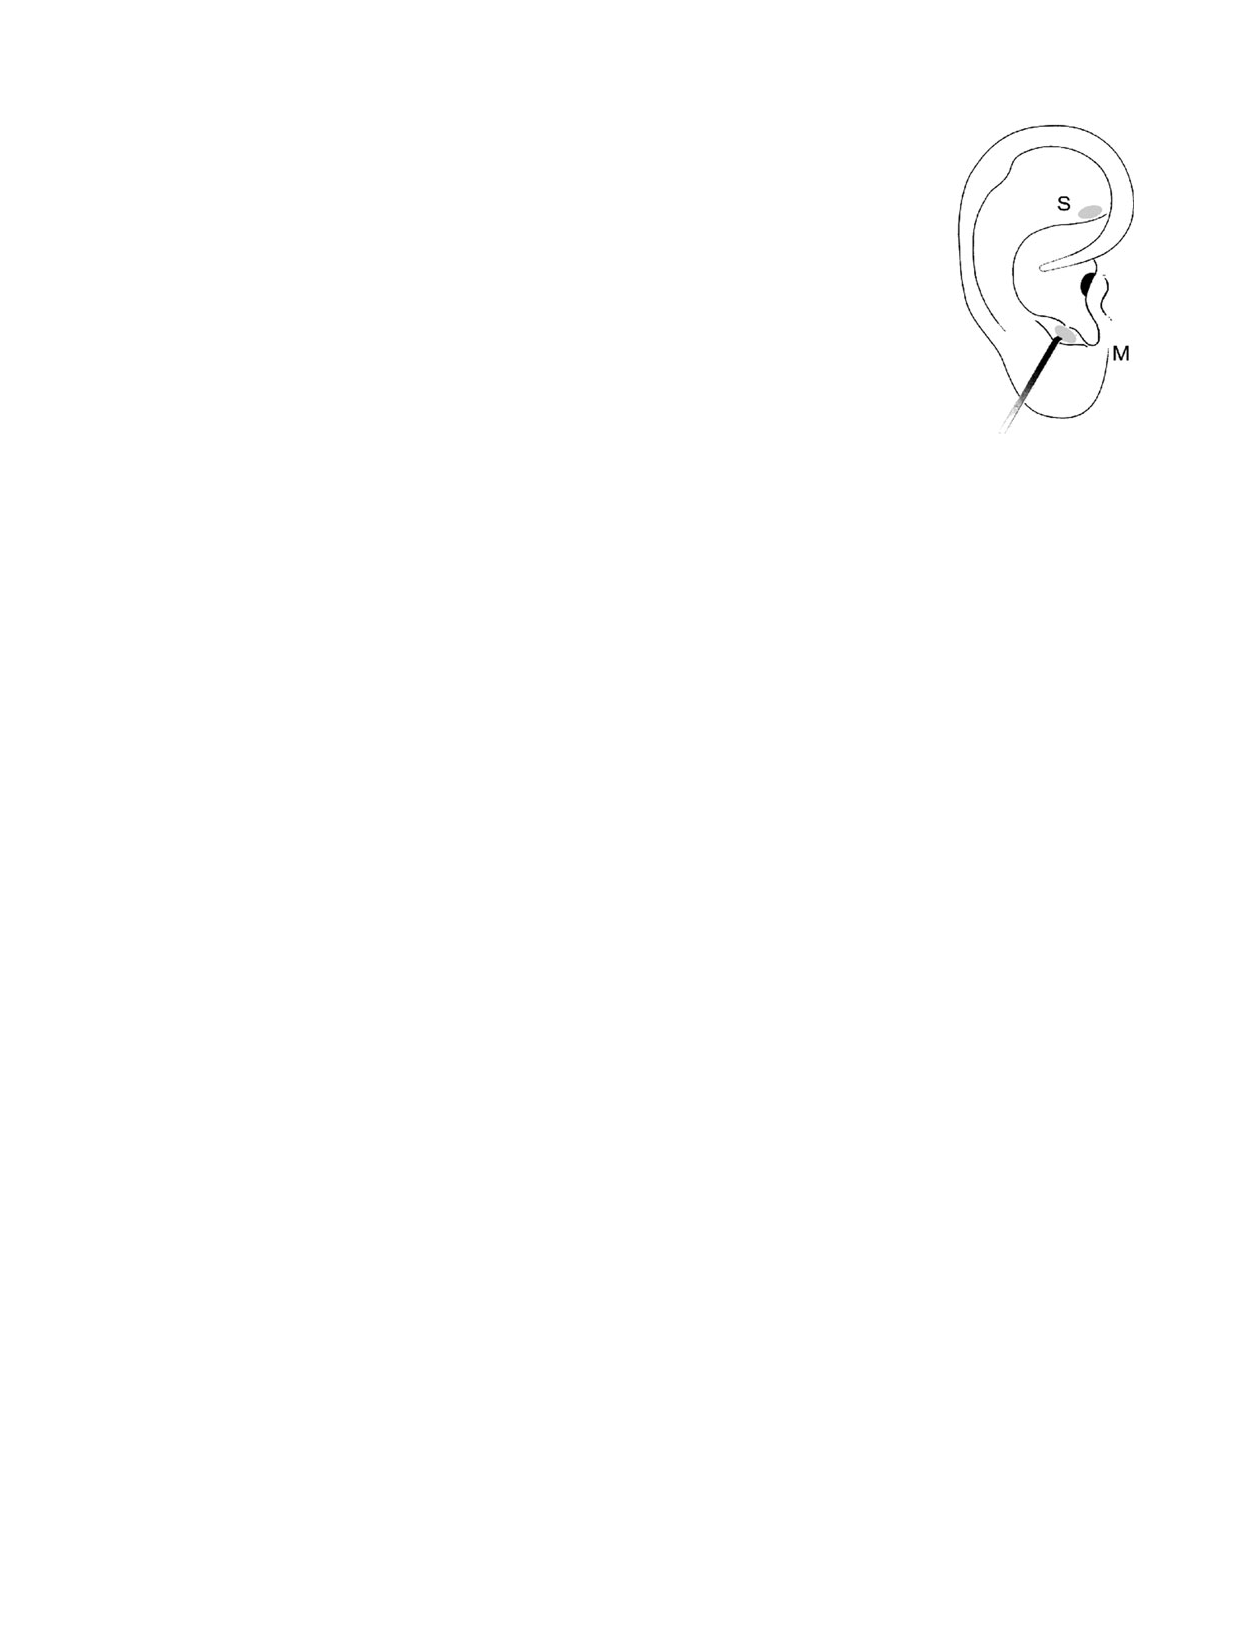
\includegraphics[width = 0.75\textwidth]{ch_data_collection/figures/eoce/migraine_and_acupuncture_intro/earacupuncture.pdf}
\end{center}
\end{minipage}
\begin{minipage}[c]{0.25\textwidth}
{\footnotesize Figure from the original paper displaying the appropriate area 
(M) versus the inappropriate area (S) used in the treatment of migraine attacks.}
\end{minipage}
\begin{parts}
\item What percent of patients in the treatment group were pain free 24 hours 
after receiving acupuncture? 
\item What percent were pain free in the control group?
\item In which group did a higher percent of patients become pain free 24 hours 
after receiving acupuncture?
\item Your findings so far might suggest that acupuncture is an effective treatment 
for migraines for all people who suffer from migraines. However this is not the 
only possible conclusion that can be drawn based on your findings so far. What is 
one other possible explanation for the observed difference between the percentages 
of patients that are pain free 24 hours after receiving acupuncture in the two groups?
\end{parts}
}{}

% 2 - sinusitis_and_antibiotics_intro

\eoce{\qt{Sinusitis and antibiotics,
    Part I\label{sinusitis_and_antibiotics_intro}} 
Researchers studying the effect of antibiotic treatment for acute sinusitis 
compared to symptomatic treatments randomly assigned 166 adults diagnosed 
with acute sinusitis to one of two groups: treatment or control. Study 
participants received either a 10-day course of amoxicillin (an antibiotic) 
or a placebo similar in appearance and taste. The placebo consisted of 
symptomatic treatments such as acetaminophen, nasal decongestants, etc.
At the end of the 10-day period, patients were asked if
they experienced improvement in symptoms.
The distribution of responses is summarized below. 
\footfullcite{Garbutt:2012}
\begin{center}
\begin{tabular}{ll  cc c} 
                                    			&			& \multicolumn{2}{c}{\textit{Self-reported improvement}} \\
                                    			&			& \multicolumn{2}{c}{\textit{in symptoms}} \\
\cline{3-4}
			                        		&			& Yes 	& No 	& Total \\
\cline{2-5}
							& Treatment 	& 66		& 19		& 85 \\
\raisebox{1.5ex}[0pt]{\emph{Group}}	& Control		& 65		& 16 		& 81 \\
\cline{2-5}
							& Total		& 131	& 35		& 166
\end{tabular}
\end{center}
\begin{parts}
\item What percent of patients in the treatment group experienced improvement 
in symptoms? 
\item What percent experienced improvement in symptoms in the 
control group?
\item In which group did a higher percentage of patients experience improvement
in symptoms?
\item Your findings so far might suggest that a real difference in effectiveness of 
antibiotic and placebo treatments for improving symptoms of sinusitis. However this is 
not the only possible conclusion that can be drawn based on your findings so far. What is 
one other possible explanation for the observed difference between the percentages 
of patients that are pain free 24 hours after receiving acupuncture in the two groups?
\end{parts}
}{}
}

%______________________________________________
\section[Data basics]{Data basics }
\label{dataBasics}
\sectionintro{
\noindent%
You collect data on dozens of questions from all of the students at your school.
How would you organize all of this data?
Effective presentation and description of data is a first step in most analyses.
This section introduces one structure for organizing data as well as some terminology that will be used throughout this book.
We use loan data from Lending Club and county data from the US Census Bureau to motivate and illustrate this section's learning objectives.


%%
\subsection*{Learning objectives}
\begin{enumerate}
\setlength{\itemsep}{0mm}
\item Identify the individuals and the variables of a study.
 
\item Identify variables as categorical or numerical.  Identify numerical variables as discrete or continuous.
 
\item Understand what it means for two variables to be associated. 
  
\end{enumerate}
}

%%

\subsection{Observations, variables, and data matrices}

\index{data!loan50|(}

Figure~\ref{loan50DF} displays rows 1, 2, 3, and 50 of a data set
for 50 randomly sampled loans offered through Lending Club,
which is a peer-to-peer lending company.
These observations will be referred to as the
\data{loan50} data set.

Each row in the table represents a single loan.
The formal name for a row is a \term{case}
or \term{observational unit}\index{unit of observation}.
The columns represent characteristics,
called \termsub{variables}{variable},
for each of the loans.
For example, the first row represents a loan of \$7,500 with an interest rate of 7.34\%, where the borrower is based in Maryland (MD) and has an income of \$70,000.

\begin{exercisewrap}
\begin{nexercise}
What is the grade of the first loan in Figure~\ref{loan50DF}?
And what is the home ownership status of the borrower
for that first loan?
For these Guided Practice questions, you can check your answer
in the footnote.\footnotemark{}
\end{nexercise}
\end{exercisewrap}
\footnotetext{The loan's grade is A,
  and the borrower rents their residence.}

In practice, it is especially important to ask clarifying
questions to ensure important aspects of the data are understood.
For instance, it is always important to be sure we know what
each variable means and the units of measurement.
Descriptions of the \data{loan50} variables are given
in Figure~\ref{loan50Variables}.

\begin{figure}[h]
\centering
{\small
\begin{tabular}{ccc ccc cc} %c}
  \hline
   & \var{loan\us{}amount}
   & \var{interest\us{}rate}
   & \var{term} & \var{grade} & \var{state}
   & \var{total\us{}income}
   & \var{homeownership} \\
  \hline
  1 & 7500 & 7.34 & 36 & A & MD & 70000 & rent \\
  2 & 25000 & 9.43 & 60 & B & OH & 254000 & mortgage \\
  3 & 14500 & 6.08 & 36 & A & MO & 80000 & mortgage \\
  $\vdots$ & $\vdots$ & $\vdots$ & $\vdots$ & $\vdots$ & $\vdots$
      & $\vdots$ & $\vdots$ \\
  50 & 3000 & 7.96 & 36 & A & CA & 34000 & rent \\
   \hline
\end{tabular}
}
\caption{Four rows from the \data{loan50} data matrix.}
\label{loan50DF}
\end{figure}
% Dropped: state, verified_income
% library(openintro); vars <- c("loan_amount", "interest_rate", "term", "grade", "total_income", "home_ownership", "loan_status"); library(xtable); data(loan50); loan50[c(1,2,3,50), vars]; xtable(loan50[c(1,2,3,50), vars])

\D{\newpage}

\begin{figure}[h]
\centering\small
\begin{tabular}{lp{10.5cm}}
\hline
{\bf variable} & {\bf description} \\
\hline
\var{loan\us{}amount} & Amount of the loan received,
    in US dollars.  \\
\var{interest\us{}rate} & Interest rate on the loan,
    in an annual percentage.  \\
\var{term} & The length of the loan, which is always set
    as a whole number of months. \\
\var{grade} & Loan grade, which takes values A through G
    and represents the quality of the loan and its likelihood
    of being repaid.  \\
\var{state} & US state where the borrower resides. \\
\var{total\us{}income} & Borrower's total income,
    including any second income, in US dollars.   \\
\var{homeownership} & Indicates whether the
    person owns, owns but has a mortgage, or rents.  \\
%\var{verified\us{}income} & Indicates whether the
%    income is verified, its source is verified but not the amount,
%    or it is not verified.   \\
\hline
\end{tabular}
\caption{Variables and their descriptions for the \data{loan50} data set.}
\label{loan50Variables}
\end{figure}

\index{data!loan50|)}

The data in Figure~\ref{loan50DF} represent a \term{data matrix},
which is a convenient and common way to organize data,
especially if collecting data in a spreadsheet.
Each row of a data matrix corresponds to a unique case
(observational unit),
and each column corresponds to a variable.
%A data matrix for the stroke study introduced in
%Section~\ref{basicExampleOfStentsAndStrokes} is shown
%in Figure~\vref{stentStudyResultsDF}, where the cases were
%patients and three variables were recorded for each
%patient.

When recording data, use a data matrix unless you have
a very good reason to use a different structure.
This structure allows new cases to be added as rows
or new variables as new columns.

\begin{exercisewrap}
\begin{nexercise}
The grades for assignments, quizzes, and exams in a course are
often recorded in a gradebook that takes the form of a data matrix.
How might you organize grade data using a data
matrix?\footnotemark
\end{nexercise}
\end{exercisewrap}

\index{data!county|(}

\begin{exercisewrap}
\begin{nexercise}\label{desc_county_as_data_matrix}%
We consider data for 3,142 counties in the United States,
which includes each county's name,
the state in which it is located, its population in 2017,
how its population changed from 2010 to 2017,
poverty rate,
and six additional characteristics.
How might these data be organized in
a data matrix?\footnotemark
\end{nexercise}
\end{exercisewrap}
\addtocounter{footnote}{-1}
\footnotetext{There are multiple strategies that can be followed.
  One common strategy is to have each student represented by a row,
  and then add a column for each assignment, quiz, or exam.
  Under this setup, it is easy to review a single line to understand
  a student's grade history.
  There should also be columns to include student information,
  such as one column to list student names.}
\addtocounter{footnote}{1}
\footnotetext{Each county may be viewed as a case,
  and there are eleven pieces of information recorded for
  each case.
  A table with 3,142 rows and 11 columns could hold these data,
  where each row represents a county and each column represents
  a particular piece of information.}

\noindent The data described in Guided
Practice~\ref{desc_county_as_data_matrix} represents the
\data{county} data set, which is shown as a data matrix
in Figure~\ref{countyDF}.
These data come from the US Census, with much of
the data coming from the US Census Bureau's American
Community Survey (ACS).
Unlike the Decennial Census, which takes place every 10 years and attempts to collect basic demographic data from every residents of the US, the ACS is an ongoing survey that is sent to approximately 3.5 million households per year.
As stated by the ACS website, these data help communities ``plan for hospitals and schools, support school lunch programs, improve emergency services, build bridges, and inform businesses looking to add jobs and expand to new markets, and more."\footnote{\oiRedirect{textbook-acs}{\url{https://www.census.gov/programs-surveys/acs/about.html}}}
A small subset of the variables from the ACS are summarized in Figure~\ref{countyVariables}.

\D{\newpage}

\begin{landscape}
\begin{figure}
\centering\small
\begin{tabular}{ccc ccc ccc ccc}
  \hline
 & \var{name} & \var{state} & \var{pop} & \var{pop\us{}change} & \var{poverty} & \var{homeownership} & \var{multi\us{}unit} & \var{unemp\us{}rate} & \var{metro} & \var{median\us{}edu} & \var{median\us{}hh\us{}income} \\ 
  \hline
1 & Autauga  & Alabama &  55504 &  1.48 & 13.7 & 77.5 &  7.2 & 3.86 & yes & some\us{}college & 55317 \\ 
  2 & Baldwin  & Alabama & 212628 &  9.19 & 11.8 & 76.7 & 22.6 & 3.99 & yes & some\us{}college & 52562 \\ 
  3 & Barbour  & Alabama &  25270 & -6.22 & 27.2 & 68.0 & 11.1 & 5.90 & no  & hs\us{}diploma   & 33368 \\ 
  4 & Bibb     & Alabama &  22668 &  0.73 & 15.2 & 82.9 &  6.6 & 4.39 & yes & hs\us{}diploma   & 43404 \\ 
  5 & Blount   & Alabama &  58013 &  0.68 & 15.6 & 82.0 &  3.7 & 4.02 & yes & hs\us{}diploma   & 47412 \\ 
  6 & Bullock  & Alabama &  10309 & -2.28 & 28.5 & 76.9 &  9.9 & 4.93 & no  & hs\us{}diploma   & 29655 \\ 
  7 & Butler   & Alabama &  19825 & -2.69 & 24.4 & 69.0 & 13.7 & 5.49 & no  & hs\us{}diploma   & 36326 \\ 
  8 & Calhoun  & Alabama & 114728 & -1.51 & 18.6 & 70.7 & 14.3 & 4.93 & yes & some\us{}college & 43686 \\ 
  9 & Chambers & Alabama &  33713 & -1.20 & 18.8 & 71.4 &  8.7 & 4.08 & no  & hs\us{}diploma   & 37342 \\ 
  10 & Cherokee & Alabama &  25857 & -0.60 & 16.1 & 77.5 &  4.3 & 4.05 & no  & hs\us{}diploma   & 40041 \\ 
  $\vdots$ & $\vdots$ & $\vdots$ & $\vdots$ & $\vdots$ & $\vdots$ & $\vdots$ & $\vdots$ & $\vdots$ & $\vdots$ & $\vdots$ & $\vdots$ \\
  3142 & Weston   & Wyoming &   6927 & -2.93 & 14.4 & 77.9 &  6.5 & 3.98 & no  & some\us{}college & 59605 \\  
   \hline
\end{tabular}
\caption{Eleven rows from the \data{county} data set.}
\label{countyDF}
% library(openintro); data(county); county$name <- gsub(" County$", "", county$name); county$pop <- county$pop2017; county$unemp_rate = county$unemployment_rate; these <- c("name", "state", "pop", "pop_change", "poverty", "homeownership", "multi_unit", "unemp_rate", "metro", "median_edu", "median_hh_income"); county <- county[, these]; library(xtable); xtable(as.data.frame(lapply(rbind.data.frame(head(county, 10), tail(county, 1)), function(x) { format(x) })))
\end{figure}

\begin{figure}
\centering\small
\begin{tabular}{lp{11cm}}
\hline
{\bf variable} & {\bf description} \\
\hline
\var{name} &
    County name. \\
\var{state} &
    State where the county resides,
    or the District of Columbia. \\
\var{pop} &
    Population in 2017. \\
\var{pop\us{}change} &
    Percent change in the population from 2010 to 2017.
    For example, the value \resp{1.48} in the first row
    means the population for this county
    increased by 1.48\% from 2010 to 2017. \\
\var{poverty} &
    Percent of the population in poverty. \\
\var{homeownership}  &
    Percent of the population that lives in their own home
    or lives with the owner, e.g. children living with parents
    who own the home. \\
\var{multi\us{}unit}  &
    Percent of living units that are in multi-unit structures,
    e.g. apartments. \\
\var{unemp\us{}rate} &
    Unemployment rate as a percent. \\
\var{metro} &
    Whether the county contains a metropolitan area. \\
\var{median\us{}edu} & Median education level, which
    can take a value among
    \resp{below\us{}hs},
    \resp{hs\us{}diploma},
    \resp{some\us{}college},
    and \resp{bachelors}. \\
\var{median\us{}hh\us{}income} &
    Median household income for the county, where a household's
    income equals the total income of its occupants who are
    15~years or older. \\
%\var{per\us{}capita\us{}income} &
%    Per capita (per person) income for the county. \\
\hline
\end{tabular}
\centering
\caption{Variables and their descriptions for the \data{county} data set.}
\label{countyVariables}
\end{figure}
\end{landscape}

\subsection{Types of variables}
\label{variableTypes}

Examine the \var{unemp\us{}rate}, \var{pop}, \var{state},
and \var{median\us{}edu} variables in the \data{county}
data set. Each of these variables is inherently different from the
other three, yet some share certain characteristics.

First consider \var{unemp\us{}rate},
which is said to be a \term{numerical} variable since
it can take a wide range of numerical values,
and it is sensible to add, subtract, or take averages
with those values.
On the other hand, we would not classify a variable
reporting telephone area codes as numerical since the
average, sum, and difference of area codes doesn't have
any clear meaning.

The \var{pop} variable is also numerical, although it seems
to be a little different than \var{unemp\us{}rate}.
This variable of the population count can only take whole
non-negative numbers (\resp{0}, \resp{1}, \resp{2}, ...).
For~this reason, the population variable is said to be
\term{discrete} since it can only take numerical values
with jumps.
On the other hand, the unemployment rate variable is said
to be \term{continuous}.

The variable \var{state} can take up to 51 values after
accounting for Washington, DC: \resp{AL}, \resp{AK}, ...,
and \resp{WY}.
Because the responses themselves are categories,
\var{state} is called a \term{categorical} variable,
and the possible values are called the variable's \term{levels}.

Finally, consider the \var{median\us{}edu} variable,
which describes the median education level of county
residents and takes values
\resp{below\us{}hs}, \resp{hs\us{}diploma},
\resp{some\us{}college}, or \resp{bachelors}
in each county.
This variable seems to be a hybrid: it is a categorical variable
but the levels have a natural ordering.
A variable with these properties is called an \term{ordinal}
variable, while a regular categorical variable without this
type of special ordering is called a \term{nominal} variable.
To simplify analyses, any ordinal variable in this book will
be treated as a nominal (unordered) categorical variable.

\begin{figure}[h]
  \centering
  \Figure{0.57}{variables}
  \caption{Breakdown of variables into their respective types.}
  \label{variables}
\end{figure}

\begin{examplewrap}
\begin{nexample}{Data were collected about students
    in a statistics course.
    Three variables were recorded for each student:
    number of siblings, student height, and whether
    the student had previously taken a statistics course.
    Classify each of the variables as continuous numerical,
    discrete numerical, or categorical.}
  The number of siblings and student height represent
  numerical variables.
  Because the number of siblings is a count, it is discrete.
  Height varies continuously, so it is a continuous numerical
  variable.
  The last variable classifies students into two categories
  -- those who have and those who have not taken a statistics
  course -- which makes this variable categorical.
\end{nexample}
\end{examplewrap}

\begin{exercisewrap}
\begin{nexercise}\index{data!stroke}%
An experiment is evaluating the effectiveness of a new drug
in treating migraines.
A \var{group} variable is used to indicate the experiment group
for each patient: treatment or control.
The \mbox{\var{num\us{}migraines}} variable represents the number
of migraines the patient experienced during a 3-month period.
\mbox{Classify} each variable as either numerical or
categorical.\footnotemark
\end{nexercise}
\end{exercisewrap}
\footnotetext{The
  \var{group} variable can take just one of two group names,
  making it categorical.
  The \var{num\us{}migraines} variable describes
  a count of the number of migraines, which is an outcome where
  basic arithmetic is sensible, which means this is a numerical
  outcome; more specifically, since it represents a count,
  \var{num\us{}migraines} is a discrete numerical variable.}


\D{\newpage}

\subsection{Relationships between variables}
\label{variableRelations}

Many analyses are motivated by a researcher looking
for a relationship between two or more variables.
A social scientist may like to answer some of the
following questions:
\newcommand{\popchangevmedianhhincomequestion}[0]{
    % Note that this question is used to introduce the
    %explanatory / response variable topic.
    Does a higher than average increase in county population
    tend to correspond to counties with higher or lower median
    household incomes?}%
\begin{enumerate}
\setlength{\itemsep}{0mm}
\item[(1)]\label{ownershipMultiUnitQuestion}
    If homeownership is lower than the national average
    in one county, will the percent of multi-unit structures
    in that county tend to be above or below the national average?
\item[(2)]\label{pop_change_v_median_hh_income_question}
    \popchangevmedianhhincomequestion{}
    % Do counties with a higher median household income
    % tend to be growing faster or slower than other counties?
\item[(3)]\label{isAverageIncomeAssociatedWithSmokingBans}
    How useful a predictor is median education level
    for the median household income for US counties?
\end{enumerate}

To answer these questions, data must be collected, such
as the \data{county} data set shown in Figure~\ref{countyDF}.
Examining summary statistics \index{summary statistic} could
provide insights for each of the three questions about counties.
Additionally, graphs can be used to visually explore the data.

\indexthis{Scatterplots}{scatterplot} are one type of graph
used to study the relationship between two numerical variables.
Figure~\ref{multiunitsVsOwnership} compares the variables
\var{homeownership} and
\var{multi\us{}unit},
which is the percent of units in multi-unit structures
(e.g. apartments, condos).
Each point on the plot represents a single county.
For instance, the highlighted dot corresponds to
County~413 in the \data{county} data set:
Chattahoochee County, Georgia, which has 39.4\% of
units in multi-unit structures and a homeownership rate
of 31.3\%.
The scatterplot suggests a relationship between the
two variables: counties with a higher rate of multi-units
tend to have lower homeownership rates.
We might brainstorm as to why this relationship exists
and investigate the ideas to determine which are the most
reasonable explanations.

\begin{figure}[h]
  \centering 
\oiRedirect{tableau-scatterplotschoose}{
  \Figure{0.79}{multiunitsVsOwnership}}
  \caption{A scatterplot of homeownership versus the percent
      of units that are in multi-unit structures for US counties.
      The highlighted dot represents Chattahoochee County, Georgia,
      which has a multi-unit rate of 39.4\% and a homeownership rate
      of 31.3\%. Explore this scatterplot and dozens of other scatterplots using American Community Survey data on Tableau Public\tableauhref{tableau-scatterplotschoose}.}
  \label{multiunitsVsOwnership}
\end{figure}

The multi-unit and homeownership rates are said to be
associated because the plot shows a discernible pattern.
When two variables show some connection with one another,
they are called \term{associated} variables.
Associated variables can also be called \term{dependent}
variables and vice-versa.

\D{\newpage}

\begin{exercisewrap}
\begin{nexercise}
Examine the variables in the \data{loan50} data set,
which are described in Figure~\vref{loan50Variables}.
Create two questions about possible relationships
between variables in \data{loan50} that are of interest
to~you.\footnotemark
\end{nexercise}
\end{exercisewrap}
\footnotetext{Two example questions:
  (1)~What is the relationship between loan amount and
      total income?
  (2)~If someone's income is above the average, will their
      interest rate tend to be above or below the average?}

\begin{examplewrap}
\begin{nexample}{This example examines the relationship
    between a county's population change
    from 2010 to 2017
    and median household income,
    which is visualized as a scatterplot in
    Figure~\ref{pop_change_v_med_income}.
    Are these variables associated?}
  The larger the median household income for a county,
  the higher the population growth observed for the county.
  While this trend isn't true for every county,
  the trend in the plot is evident.
  Since there is some relationship between the variables,
  they are associated.
\end{nexample}
\end{examplewrap}

%When two variables show some connection with one another,
%they are called \term{associated} variables.
%Associated variables can also be called \term{dependent}
%variables and vice-versa.
%When the variables increase together,
%as they do in Figure~\ref{loan_amount_vs_income},
%they are said to be \term{positively associated}.
%When the trend in the scatterplot goes down to the right,
%then they are described as \term{negatively correlated}.

%While we may find it interesting to consider the relationship
%between two variables such as those in the scatterplot,
%the relationship between those variables can be more complex.
%For example, interest rates on loans tend to be chosen based
%on the riskiness of the loan, i.e. how likely it is to be
%paid back, and that is likely to depend on a variety of
%details, such as what the loan is for, the person's
%creditworthiness, whether their income is verified, etc.
%We will begin exploring some of these more complex relationships
%in graphs in Chapter~\ref{ch_summarizing_data} and beyond.
%\Comment{Revise if we don't add these more rich plots...}

%\begin{example}{Figure~\ref{interest_rate_vs_loan_amount}
%    features a scatterplot of interest rate against loan amount.
%    Are these variables associated?}
%  There isn't an evident trend in the data,
%  so we would say these two variables are not associated.
%\end{example}

\begin{figure}
  \centering
\oiRedirect{tableau-scatterplotschoose}{
  \Figure{0.9}{pop_change_v_med_income}
}
  \caption{A scatterplot showing
      \var{pop\us{}change}
      against \var{median\us{}hh\us{}income}.
      Owsley County of Kentucky, is highlighted,
      which lost 3.63\% of its population from 2010 to 2017
      and had median household income of \$22,736.  Explore this scatterplot and dozens of other scatterplots using American Community Survey data on Tableau Public\tableauhref{tableau-scatterplotschoose}.}
  \label{pop_change_v_med_income}
\end{figure}

Because there is a downward trend in
Figure~\ref{multiunitsVsOwnership} --
counties with more units in multi-unit structures
are associated with lower homeownership --
these variables are said to be
\termsub{negatively associated}{negative association}.
A~\term{positive association} is shown in the relationship
between the
\var{median\us{}hh\us{}income}
and \var{pop\us{}change}
in Figure~\ref{pop_change_v_med_income},
where counties with higher median household income tend
to have higher rates of population growth.

If two variables are not associated,
then they are said to be \term{independent}.
That is, two variables are independent if there
is no evident relationship between the two.

\begin{onebox}{Associated or independent, not both}
A pair of variables is either related in some way (associated) or not (independent). No pair of variables is both associated and independent.
\end{onebox}



\index{data!county|)}



\D{\newpage}

%%
\subsection*{Section summary}
\begin{itemize}
\item Researchers often summarize data in a table, where the rows correspond to individuals or \term{cases} and the columns correspond to the \termsub{variables}{variable}, the values of which are recorded for each individual.

\item Variables can be \term{numerical} (measured on a numerical scale) or \term{categorical} (taking on levels, such as low/medium/high).  Numerical variables can be \term{continuous}, where all values within a range are possible, or \term{discrete}, where only specific  values, usually integer values, are possible.

\item When there exists a relationship between two variables, the variables are said to be \term{associated} or \term{dependent}.  If the variables are not associated, they are said to be \term{independent}.

\end{itemize}



%%%section exercises
{\exercisesheader{}

% 3 - study_components_airpoll

\eoce{\qt{Air pollution and birth outcomes, study components\label{study_components_airpoll}} 
Researchers collected data to examine the relationship between air pollutants 
and preterm births in Southern California. During the study air pollution levels 
were measured by air quality monitoring stations. Specifically, levels of carbon 
monoxide were recorded in parts per million, nitrogen dioxide and ozone in parts 
per hundred million, and coarse particulate matter (PM$_{10}$) in $\mu g/m^3$. 
Length of gestation data were collected on 143,196 births between the years 1989 
and 1993, and air pollution exposure during gestation was calculated for each 
birth. The analysis suggested that increased ambient PM$_{10}$ and, to a lesser 
degree, CO concentrations may be associated with the occurrence of preterm births.\footfullcite{Ritz+Yu+Chapa+Fruin:2000}
\begin{parts}
\item Identify the main research question of the study.
\item Who are the subjects in this study, and how many are included?
\item What are the variables in the study? Identify each variable as numerical or 
categorical. If numerical, state whether the variable is discrete or continuous.
If categorical, state whether the variable is ordinal.
\end{parts}
}{}

% 4 - study_components_buteyko

\eoce{\qt{Buteyko method, study components\label{study_components_buteyko}} 
The Buteyko method is a shallow breathing technique developed by Konstantin 
Buteyko, a Russian doctor, in 1952. Anecdotal evidence suggests that the Buteyko 
method can reduce asthma symptoms and improve quality of life. In a scientific 
study to determine the effectiveness of this method, researchers recruited 600 
asthma patients aged 18-69 who relied on medication for asthma treatment. These 
patients were randomnly split into two research groups: one practiced the Buteyko 
method and the other did not. Patients were scored on quality of life, activity, 
asthma symptoms, and medication reduction on a scale from 0 to 10. On average, 
the participants in the Buteyko group experienced a significant reduction in 
asthma symptoms and an improvement in quality of life.\footfullcite{McDowan:2003} 
\begin{parts}
\item Identify the main research question of the study.
\item Who are the subjects in this study, and how many are included?
\item What are the variables in the study? Identify each variable as numerical or 
categorical. If numerical, state whether the variable is discrete or continuous.
If categorical, state whether the variable is ordinal.
\end{parts}
}{}

% 5 - study_components_cheaters

\eoce{\qt{Cheaters, study components\label{study_components_cheaters}} 
Researchers studying the relationship between honesty, age and self-control 
conducted an experiment on 160 children between the ages of 5 and 15. 
Participants reported their age, sex, and whether they were an only child 
or not. The researchers asked each child to toss a fair coin in private and 
to record the outcome (white or black) on a paper sheet, and said they 
would only reward children who report white.\footfullcite{Bucciol:2011} 
\begin{parts}
\item Identify the main research question of the study.
\item Who are the subjects in this study, and how many are included?
\item The study's findings can be summarized as follows: "Half the students were 
explicitly told not to cheat and the others were not given any explicit 
instructions. In the no instruction group probability of cheating was found to 
be uniform across groups based on child's characteristics. In the group that was 
explicitly told to not cheat, girls were less likely to cheat, and while rate 
of cheating didn't vary by age for boys, it decreased with age for girls." 
How many variables were recorded for each subject in the study in order to 
conclude these findings? State the variables and their types.
\end{parts}
}{}

% 6 - study_components_stealers

\eoce{\qt{Stealers, study components\label{study_components_stealers}} 
In a study of the relationship between socio-economic class and unethical 
behavior, 129 University of California undergraduates at Berkeley were asked 
to identify themselves as having low or high social-class by comparing 
themselves to others with the most (least) money, most (least) education, and 
most (least) respected jobs. They were also presented with a jar of 
individually wrapped candies and informed that the candies were for children
in a nearby laboratory, but that they could take some if they wanted. After 
completing some unrelated tasks, participants reported the number of candies 
they had taken.\footfullcite{Piff:2012} 
\begin{parts}
\item Identify the main research question of the study.
\item Who are the subjects in this study, and how many are included?
\item The study found that students who were identified as upper-class took more 
candy than others. How many variables were recorded for each subject in the study 
in order to conclude these findings? State the variables and their types.
\end{parts}
}{}

% 7 - migraine_and_acupuncture_exp_resp

\eoce{\qt{Migraine and acupuncture,
    Part II\label{migraine_and_acupuncture_exp_resp}}
Exercise~\ref{migraine_and_acupuncture_intro}
introduced a study exploring whether acupuncture had any
effect on migraines.
Researchers conducted a randomized controlled study
where patients were randomly assigned to one of two groups:
treatment or control.
The patients in the treatment group received acupuncture
that was specifically designed to treat migraines.
The patients in the control group received placebo acupuncture
(needle insertion at non-acupoint locations).
24 hours after patients received acupuncture, they were asked 
if they were pain free.
What are the explanatory and response variables in this study?
}{}

% 8 - sinusitis_and_antibiotics_exp_resp

\eoce{\qt{Sinusitis and antibiotics,
    Part II\label{sinusitis_and_antibiotics_exp_resp}} 
Exercise~\ref{sinusitis_and_antibiotics_intro}
introduced a study exploring the effect of antibiotic treatment
for acute sinusitis.
Study participants either received either a 10-day course of
an antibiotic (treatment)
or a placebo similar in appearance and taste (control).
At the end of the 10-day period, patients were asked if
they experienced improvement in symptoms.
What are the explanatory and response variables in this study?
}{}

% 9 - fisher_irises

\eoce{\qt{Fisher's irises\label{fisher_irises}} Sir Ronald Aylmer Fisher was an 
English statistician, evolutionary biologist, and geneticist who worked on a 
data set that contained sepal length and width, and petal length and width from 
three species of iris flowers (\textit{setosa}, \textit{versicolor} and 
\textit{virginica}). There were 50 flowers from each species in the data set. 
\footfullcite{Fisher:1936} \\
\noindent\begin{minipage}[c]{0.48\textwidth}
\begin{parts}
\item How many cases were included in the data?
\item How many numerical variables are included in the data? Indicate what 
they are, and if they are continuous or discrete.
\item How many categorical variables are included in the data, and what are 
they? List the corresponding levels (categories).
\end{parts}
\end{minipage}
\begin{minipage}[c]{0.01\textwidth}
\ 
\end{minipage}
\begin{minipage}[c]{0.2\textwidth}
\begin{center}
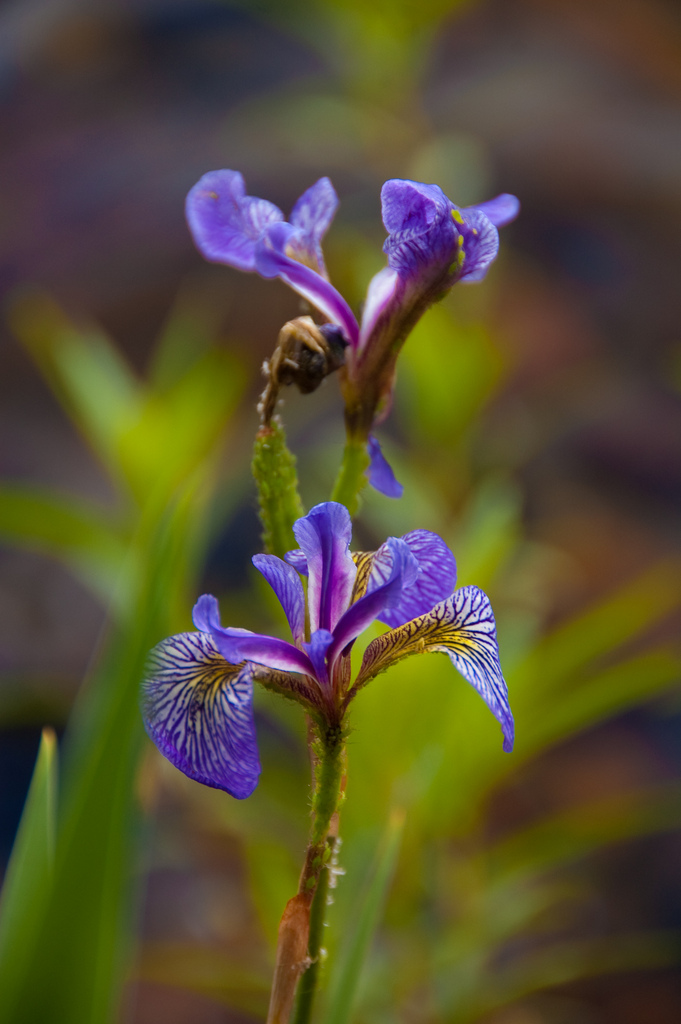
\includegraphics[width = \textwidth]{ch_data_collection/figures/eoce/fisher_irises/irisversicolor.jpg}
\end{center}
\end{minipage}
\begin{minipage}[c]{0.01\textwidth}
\ 
\end{minipage}
\begin{minipage}[c]{0.23\textwidth}
{\raggedright\footnotesize Photo by Ryan Claussen 
(\oiRedirect{textbook-flickr_ryan_claussen_iris_picture}{http://flic.kr/p/6QTcuX}) 
\oiRedirect{textbook-CC_BY_SA_2}{CC~BY-SA~2.0~license}}
\end{minipage}
}{}

% 10 - smoking_habits_UK_datamatrix

\eoce{\qt{Smoking habits of UK residents\label{smoking_habits_UK_datamatrix}} A survey 
was conducted to study the smoking habits of UK residents. Below is a data 
matrix displaying a portion of the data collected in this survey. Note that 
``$\pounds$" stands for British Pounds Sterling, ``cig" stands for cigarettes, 
and ``N/A'' refers to a missing component of the data. \footfullcite{data:smoking}
\begin{center}
\scriptsize{
\begin{tabular}{rccccccc}
\hline
	& sex 	 & age 	& marital 	& grossIncome 					     & smoke & amtWeekends	& amtWeekdays \\ 
\hline
1 	& Female & 42 	& Single 	& Under $\pounds$2,600 			     & Yes 	 & 12 cig/day   & 12 cig/day \\ 
2 	& Male	 & 44	& Single 	& $\pounds$10,400 to $\pounds$15,600 & No	 & N/A 			& N/A \\ 
3 	& Male 	 & 53 	& Married   & Above $\pounds$36,400 		     & Yes 	 & 6 cig/day 	& 6 cig/day \\ 
\vdots & \vdots & \vdots & \vdots & \vdots 				             & \vdots & \vdots 	    & \vdots \\ 
1691 & Male  & 40   & Single 	& $\pounds$2,600 to $\pounds$5,200   & Yes 	 & 8 cig/day 	& 8 cig/day \\   
\hline
\end{tabular}
}
\end{center}
\begin{parts}
\item What does each row of the data matrix represent?
\item How many participants were included in the survey?
\item Indicate whether each variable in the study is numerical or categorical. If numerical, identify as 
continuous or discrete. If categorical, indicate if the variable is ordinal.
\end{parts}
}{}

% 11 - airports

\eoce{\qt{US Airports\label{US Airports}}
The visualization below shows the
geographical distribution of airports in the contiguous United States
and Washington, DC.
This visualization was constructed based on a dataset where
each observation is an airport.\footfullcite{data:usairports}
\begin{center}
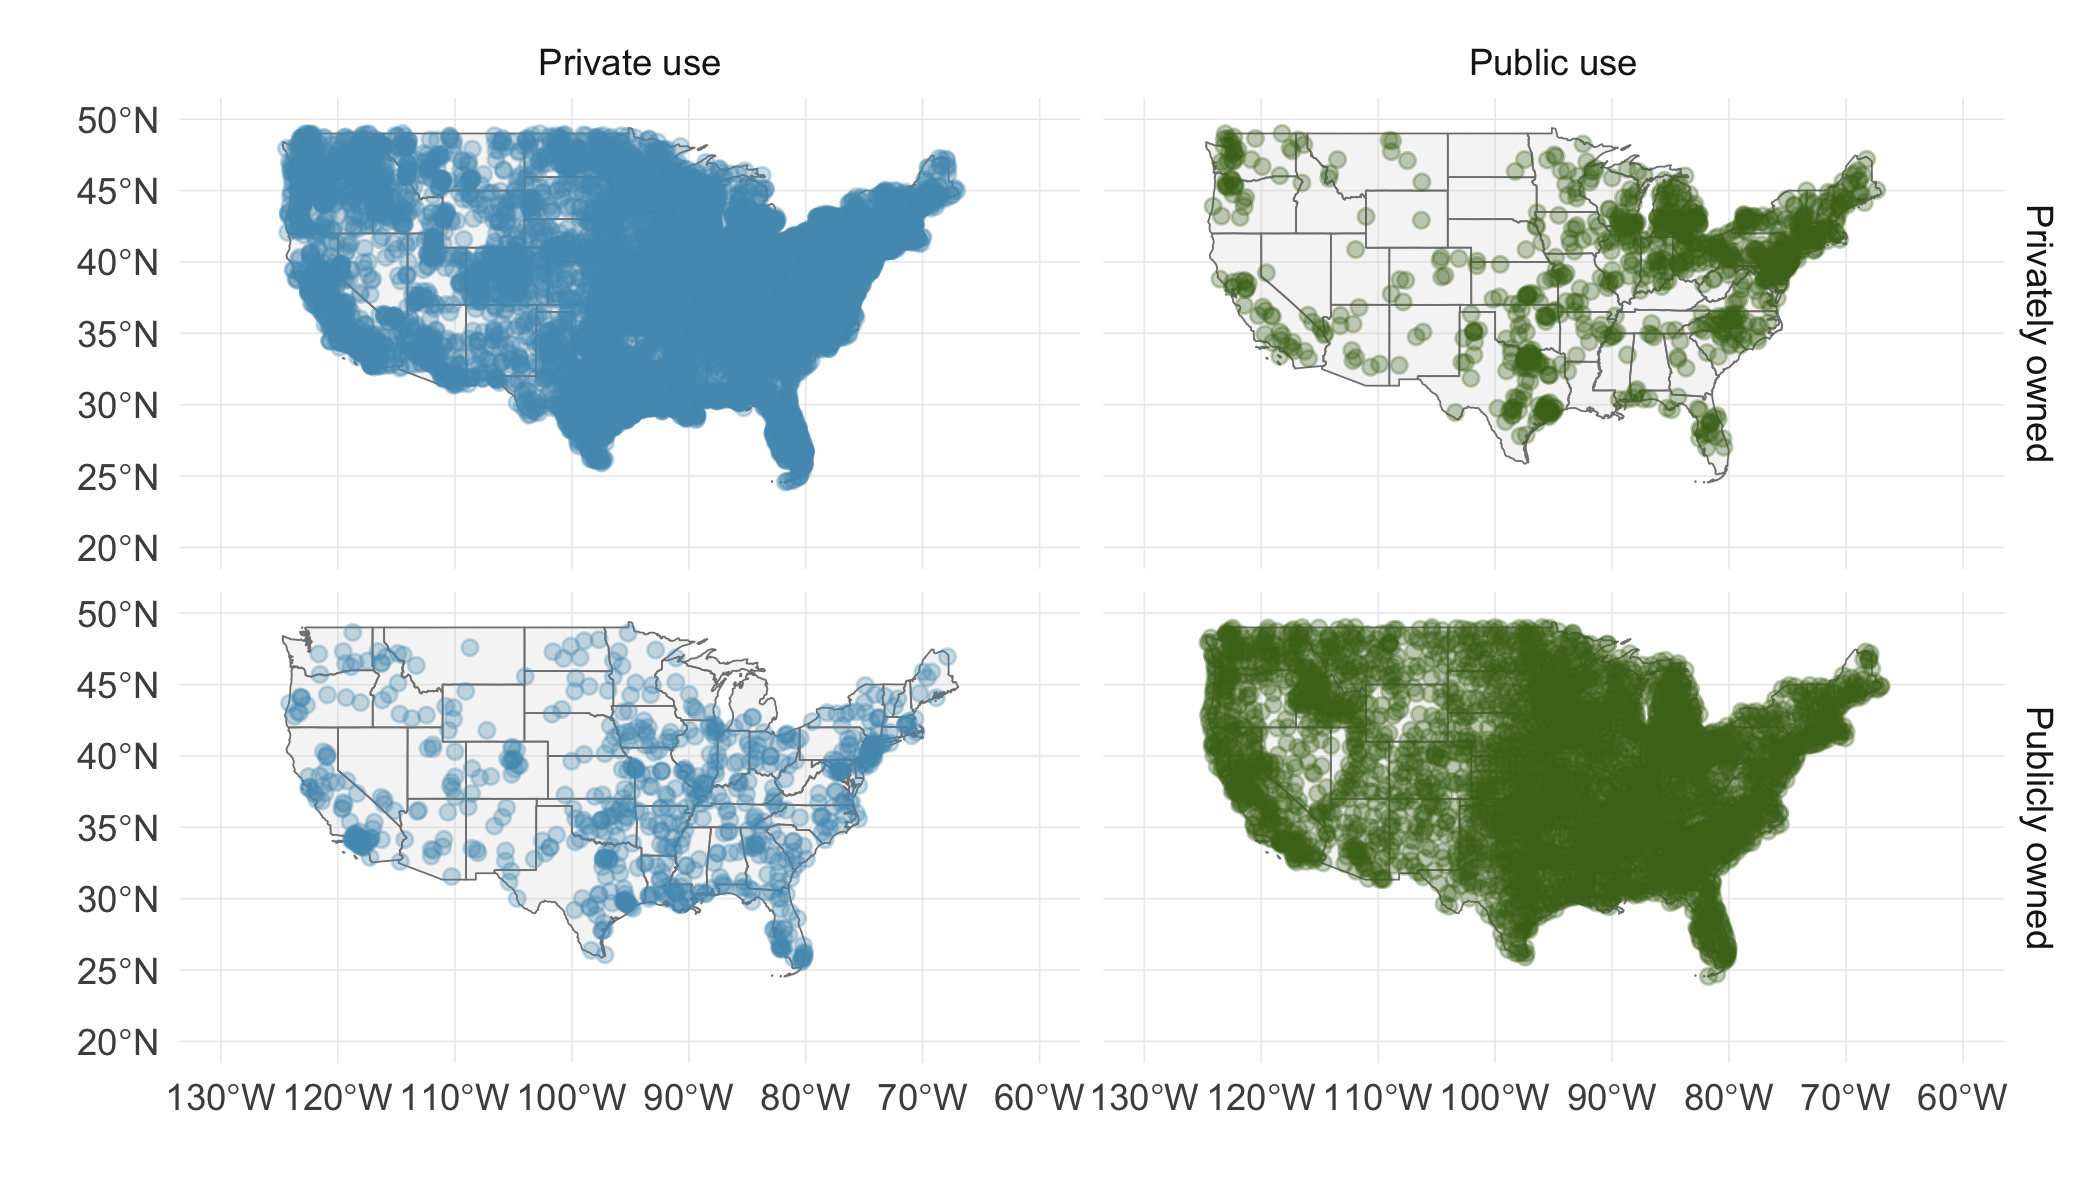
\includegraphics[width = 0.9\textwidth]{ch_data_collection/figures/eoce/airports/airports.png}
\end{center}
\begin{parts}
\item
    List the variables used in creating this visualization.
\item
    Indicate whether each variable in the study is numerical
    or categorical.
    If numerical, identify as continuous or discrete.
    If categorical, indicate if the variable is ordinal.
\end{parts}
}{}

% 12 - unvotes

\eoce{\qt{UN Votes\label{unvotes}}
The visualization below shows voting patterns 
the United States, Canada, and Mexico in the United Nations General Assembly 
on a variety of issues. Specifically, for a given year between 1946 and 2015, 
it displays the percentage of roll calls in which the country voted yes for 
each issue. This visualization was constructed based on a dataset where each 
observation is a country/year pair.\footfullcite{data:unvotes}
\begin{center}
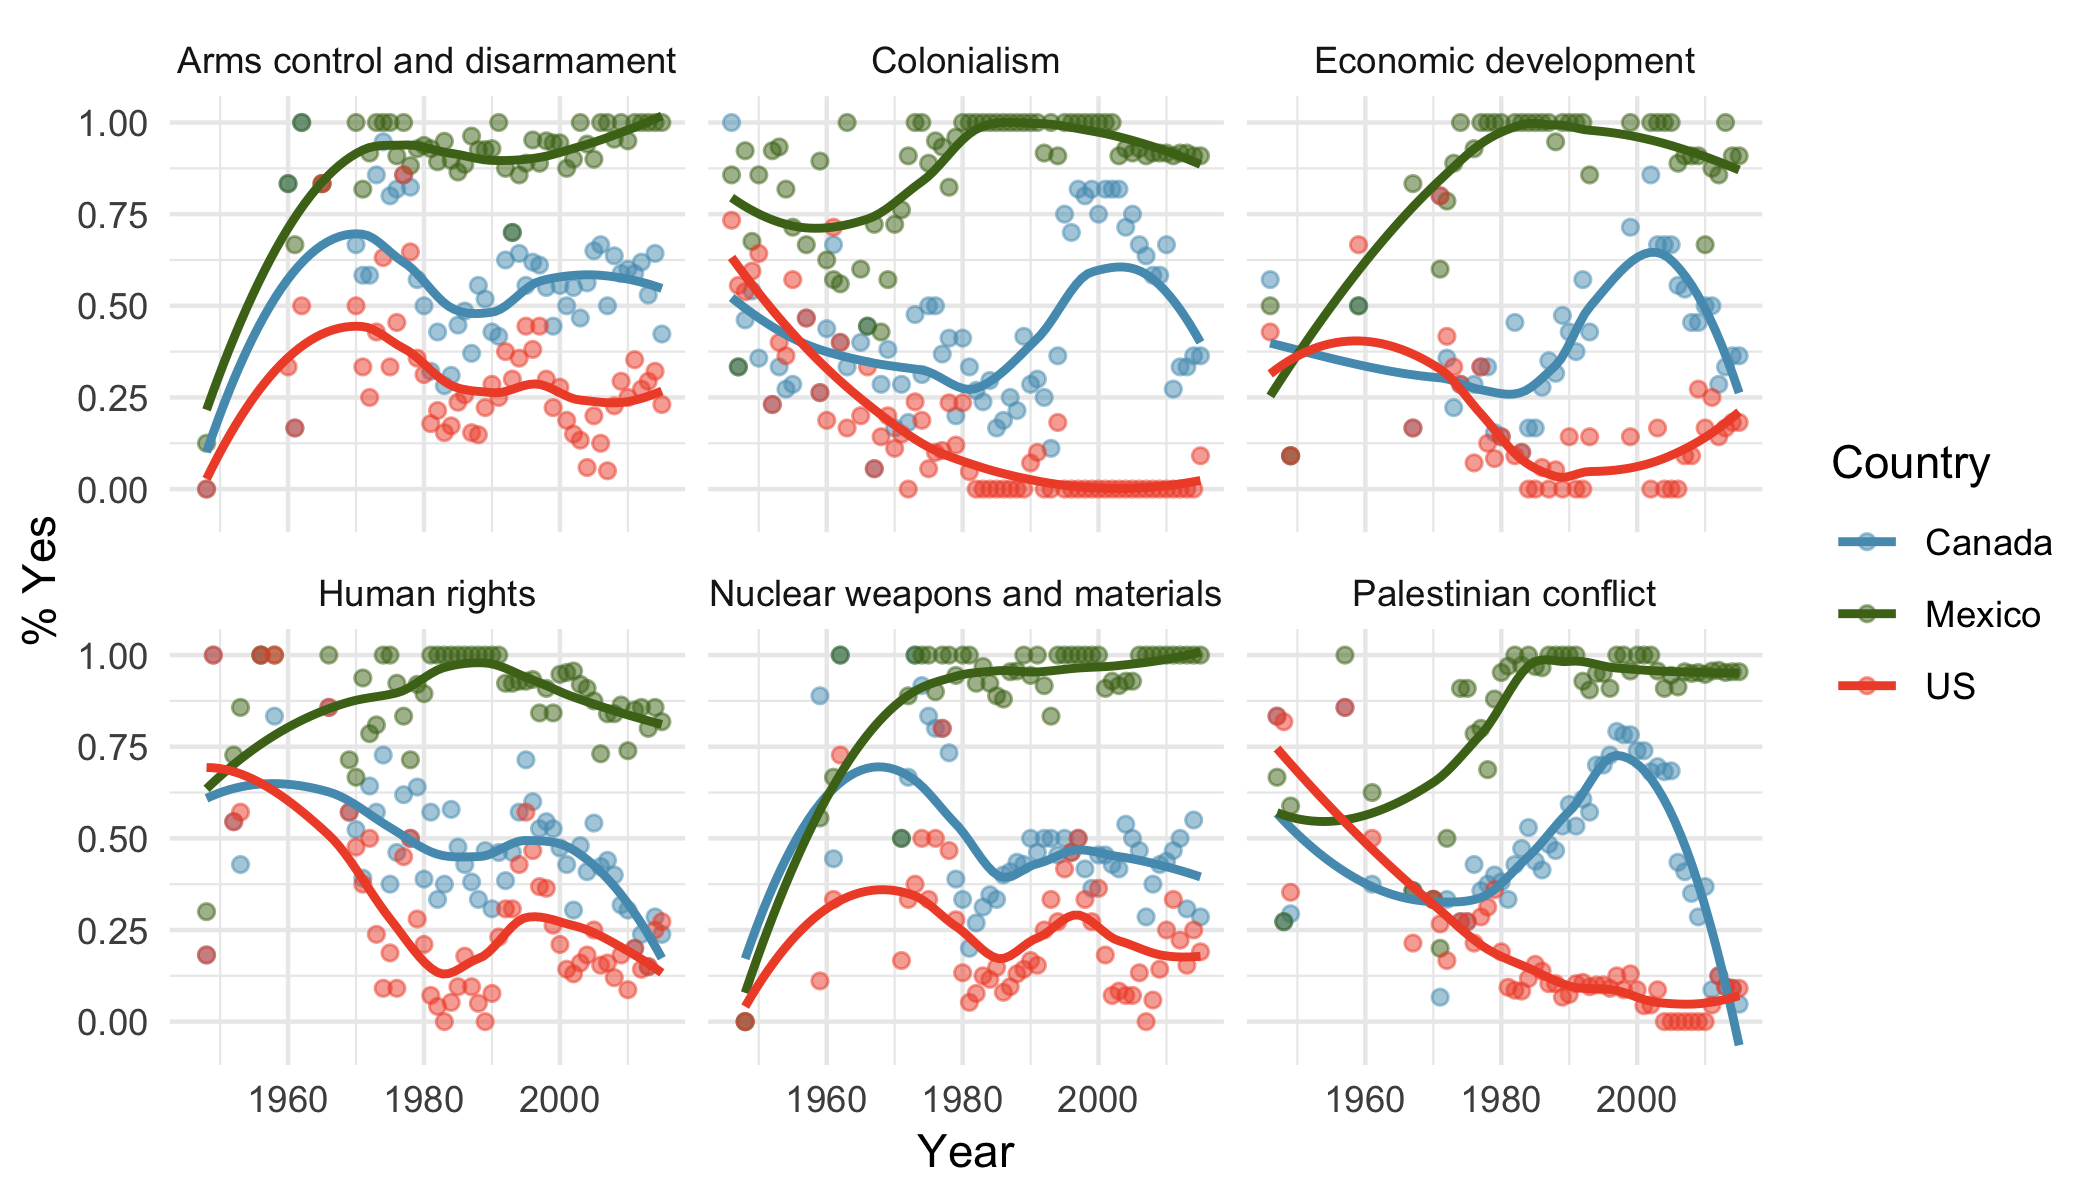
\includegraphics[width = 0.9\textwidth]{ch_data_collection/figures/eoce/unvotes/unvotes.png}
\end{center}
\begin{parts}
\item List the variables used in creating this visualization.
\item Indicate whether each variable in the study is numerical or categorical. 
If numerical, identify as continuous or discrete. If categorical, indicate if 
the variable is ordinal.
\end{parts}
}{}
}

%_______________________________
\section[Overview of data collection principles]{Overview of data collection principles }
\label{overviewOfDataCollectionPrinciples}

\index{sample|(}
\index{population|(}
\index{parameter|(}
\index{statistic|(}

\sectionintro{
\noindent%
How do researchers collect data?  Why are the results of some studies more reliable than others?
The way a researcher collects data depends upon the research goals.
In~this section, we look at different methods of collecting data and consider the types of conclusions that can be drawn from those methods.
%%
\subsection*{Learning objectives}

\begin{enumerate}
\setlength{\itemsep}{0mm}
\item Distinguish between the population and a sample and between the parameter and a statistic. 
 
\item Know when to summarize a data set using a mean versus a proportion.
 
\item Understand why anecdotal evidence is unreliable.
 
\item Identify the four main types of data collection: census, sample survey, experiment, and observation study. 
 
\item Classify a study as observational or experimental, and determine when a study's results can be generalized to the population and when a causal relationship can be drawn.

\end{enumerate}
}

%%
\subsection{Populations and samples}
\label{populationsAndSamples}

\noindent Consider the following three research questions:
\begin{enumerate}
\setlength{\itemsep}{0mm}
\item What is the average mercury content in swordfish in the Atlantic Ocean?
\item\label{timeToGraduationQuestionForUCLAStudents} Over the last 5 years, what is the average time to complete a degree for Duke undergrads?
\item\label{identifyPopulationOfStentStudy} Does a new drug reduce the number of deaths in patients with severe heart disease?
\end{enumerate}
Each research question refers to a target \term{population}. In the first question, the target population is all swordfish in the Atlantic ocean, and each fish represents a case. Often times, it is too expensive to collect data for every case in a population. Instead, a sample is taken. A \term{sample} represents a subset of the cases and is often a small fraction of the population. For instance, 60 swordfish (or some other number) in the population might be selected, and this sample data may be used to provide an estimate of the population average and answer the research question.

\begin{exercisewrap}
\begin{nexercise} \label{identifyingThePopulationForTwoQuestionsInPopAndSampSubsection}
For the second and third questions above, identify the target population and what represents an individual case.\footnotemark
\end{nexercise}
\end{exercisewrap}
\footnotetext{(\ref{timeToGraduationQuestionForUCLAStudents}) Notice that this question is only relevant to students who complete their degree; the average cannot be computed using a student who never finished her degree. Thus, only Duke undergrads who have graduated in the last five years are part of the population of interest. Each such student would represent an individual case. (\ref{identifyPopulationOfStentStudy}) A person with severe heart disease represents a case. The population includes all people with severe heart disease.}

\D{\newpage}

We collect a sample of data to better understand the characteristics of a population. A \term{variable} is a characteristic we measure for each individual or case. The overall quantity of interest may be the mean, median, proportion, or some other summary of a population. These population values are called \termsub{parameters}{parameter}. We estimate the value of a parameter by taking a sample and computing a numerical summary called a \term{statistic} based on that sample. Note that the two p's (population, parameter) go together and the two s's (sample, statistic) go together.

\begin{examplewrap}
\begin{nexample}{Earlier we asked the question: what is the average mercury content in swordfish in the Atlantic Ocean? Identify the variable to be measured and the parameter and statistic of interest.}The variable is the level of mercury content in swordfish in the Atlantic Ocean. It will be measured for each individual swordfish. The parameter of interest is the average mercury content in \emph{all} swordfish in the Atlantic Ocean. If we take a sample of 50 swordfish from the Atlantic Ocean, the average mercury content among just those 50 swordfish will be the statistic.
\end{nexample}
\end{examplewrap}

Two statistics we will study are the \term{mean} (also called the \term{average}) and \term{proportion}. When we are discussing a population, we label the mean as $\mu$ (the Greek letter, \emph{mu}), while we label the sample mean as $\bar{x}$ (read as \emph{x-bar}). When we are discussing a proportion in the context of a population, we use the label $p$, while the sample proportion has a label of $\hat{p}$ (read as \emph{p-hat}). Generally, we use $\bar{x}$ to estimate the population mean, $\mu$. Likewise, we use the sample proportion $\hat{p}$ to estimate the population proportion, $p$.

\begin{examplewrap}
\begin{nexample}{Is $\mu$ a parameter or statistic? What about $\hat{p}$?}$\mu$ is a parameter because it refers to the average of the \emph{entire} population. $\hat{p}$ is a statistic because it is calculated from a sample.
\end{nexample}
\end{examplewrap}

\begin{examplewrap}
\begin{nexample}{For the second question regarding time to complete a degree for a Duke undergraduate, is the variable numerical or categorical? What is the parameter of interest?}
The characteristic that we record on each individual is the number of years until graduation, which is a numerical variable. The parameter of interest is the average time to degree for all Duke undergraduates, and we use $\mu$ to describe this quantity.
\end{nexample}
\end{examplewrap}

\begin{exercisewrap}
\begin{nexercise}The third question asked whether a new drug reduces deaths in patients with severe heart disease. Is the variable numerical or categorical? Describe the statistic that should be calculated in this study.\footnotemark
\end{nexercise}
\end{exercisewrap}
\footnotetext{The variable is whether or not a patient with severe heart disease dies within the time frame of the study. This is categorical because it will be a yes or a no. The statistic that should be recorded is the proportion of patients that die within the time frame of the study, and we would use $\hat{p}$ to denote this quantity.}

If these topics are still a bit unclear, don't worry. We'll cover them in greater detail in the next chapter.


\D{\newpage}

%%
\subsection{Anecdotal evidence}
\label{anecdotalEvidenceSubsection}

Consider the following possible responses to the three research questions:
\begin{enumerate}
\item A man on the news got mercury poisoning from eating swordfish, so the average mercury concentration in swordfish must be dangerously high.
\item\label{iKnowThreeStudentsWhoTookMoreThan7YearsToGraduateAtDuke} I met two students who took more than 7~years to graduate from Duke, so it must take longer to graduate at Duke than at many other colleges.
\item\label{myFriendsDadDiedAfterSulphinpyrazon} My friend's dad had a heart attack and died after they gave him a new heart disease drug, so the drug must not work.
\end{enumerate}
Each conclusion is based on data. However, there are two problems. First, the data only represent one or two cases. Second, and more importantly, it is unclear whether these cases are actually representative of the population. Data collected in this haphazard fashion are called \term{anecdotal evidence}.

\setlength{\captionwidth}{\textwidth-80mm}
\begin{figure}
\centering
\hspace{8mm}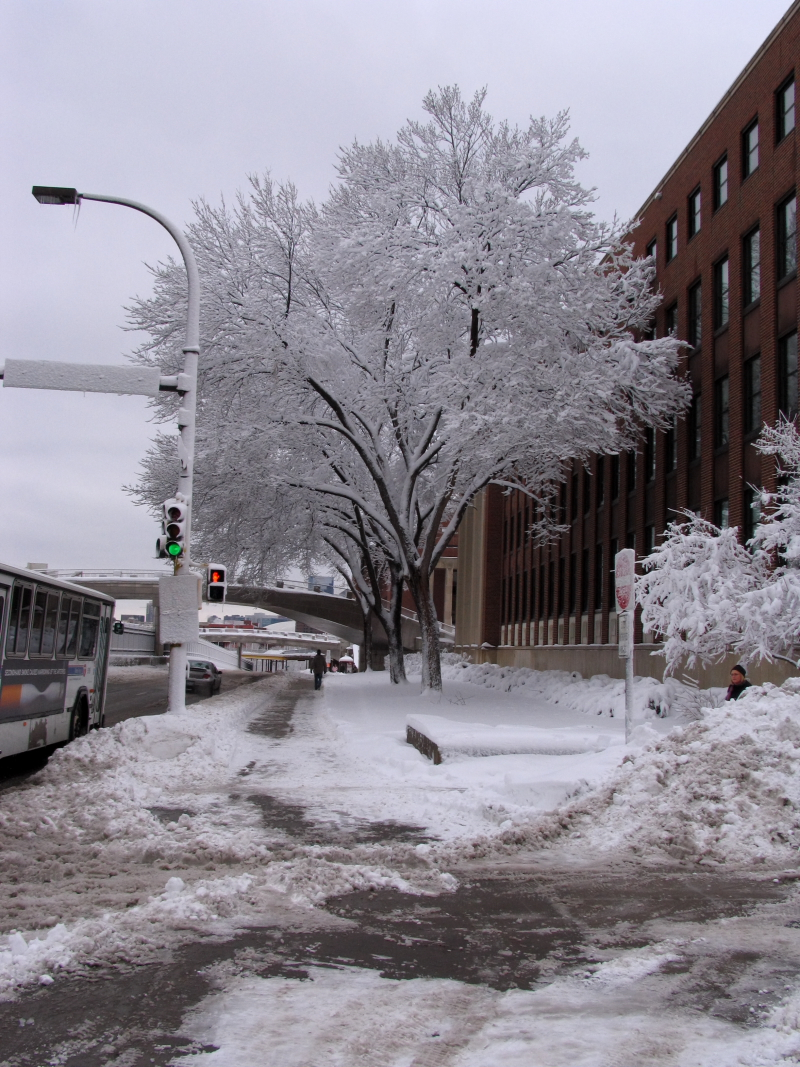
\includegraphics[width=60mm]{ch_data_collection/figures/mnWinter/mnWinter}\hspace{4mm}
\begin{minipage}[b]{\textwidth - 80mm}
   \caption[anecdotal evidence]{In February 2010, some media pundits cited one large snow storm as valid evidence against global warming. As comedian Jon Stewart pointed out, ``It's one storm, in one region, of one country.''\vspace{-4.5mm} \\

   -----------------------------\vspace{-2mm}\\
   {\footnotesize February 10th, 2010.}
   \label{mnWinter}}
\end{minipage}
\end{figure}
\setlength{\captionwidth}{\mycaptionwidth}

\begin{onebox}{Anecdotal evidence}
Be careful of making inferences based on anecdotal evidence. Such evidence may be true and verifiable, but it may only represent extraordinary cases. The majority of cases and the average case may in fact be very different.\end{onebox}

Anecdotal evidence typically is composed of unusual cases that we recall based on their striking characteristics. For instance, we may vividly remember the time when our friend bought a lottery ticket and won \$250 but forget most the times she bought one and lost. Instead of focusing on the most unusual cases, we should examine a representative sample of many cases.


\D{\newpage}

%%
\subsection{Explanatory and response variables}
\label{explanatoryAndResponse}

\index{data!county|(}

When we ask questions about the relationship
between two variables, we sometimes also want to determine
if the change in one variable causes a change in the other.
Consider the following rephrasing of an earlier question
about the \data{county} data set:
\begin{quote}\em
  If there is an increase in the median household income
  in a county, does this drive an increase in its population?
\end{quote}
In this question, we are asking whether one variable
affects another.
If this is our underlying belief,
then \emph{median household income} is the
\termsub{explanatory}{explanatory variable}
variable and the \emph{population change} is the
\termsub{response}{response variable} variable
in the hypothesized relationship.\footnote{Sometimes
  the explanatory variable is called the \term{independent}
  variable and the response variable is called the
  \term{dependent} variable.
  However, this becomes confusing since a \emph{pair}
  of variables might be independent or dependent,
  so we avoid this language.}

\index{data!county|)}

\begin{onebox}{Explanatory and response variables}
When we suspect one variable might causally affect another,
we label the first variable the explanatory variable and the
second the response variable.
\vspace{1mm}

\hspace{10mm}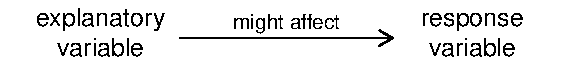
\includegraphics[height=0.34in]{ch_data_collection/figures/expResp/expResp}

For many pairs of variables, there is no hypothesized
relationship, and these labels would not be applied to
either variable in such cases.
\end{onebox}

\begin{onebox}{Association does not imply causation}
{Labeling variables as \emph{explanatory} and \emph{response} does not guarantee the relationship between the two is actually causal, even if there is an association identified between the two variables. We use these labels only to keep track of which variable we suspect affects the other.}
\end{onebox}

In many cases, the relationship is complex or unknown. It may be unclear whether variable $A$ explains variable $B$ or whether variable $B$ explains variable $A$. For example, it is now known that a particular protein called REST is much depleted in people suffering from Alzheimer's disease. While this raises hopes of a possible approach for treating Alzheimer's, it is still unknown whether the lack of the protein causes brain deterioration, whether brain deterioration causes depletion in the REST protein, or whether some third variable causes both brain deterioration and REST depletion. That~is, we do not know if the lack of the protein is an explanatory variable or a response variable. Perhaps it is both.\footnote{\oiRedirect{textbook-nytimes_gene_alzheimers_study}{nytimes.com/2014/03/20/health/fetal-gene-may-protect-brain-from-alzheimers-study-finds.html}}


\D{\newpage}

%%
\subsection{Observational studies versus experiments}

\noindent There are two primary types of data collection: observational studies and experiments.

Researchers perform an \term{observational study} when they collect data without interfering with how the data arise. For instance, researchers may collect information via surveys, review medical or company records, or follow a \term{cohort} of many similar individuals to study why certain diseases might develop. In each of these situations, researchers merely observe or take measurements of things that arise naturally.

When researchers want to investigate the possibility of a causal connection, they conduct an \term{experiment}. For all experiments, the researchers must impose a treatment. For most studies there will be both an explanatory and a response variable. For instance, we may suspect administering a drug will reduce mortality in heart attack patients over the following year. To check if there really is a causal connection between the explanatory variable and the response, researchers will collect a sample of individuals and split them into groups. The individuals in each group are \emph{assigned} a treatment. When individuals are randomly assigned to a group, the experiment is called a \term{randomized experiment}. For example, each heart attack patient in the drug trial could be randomly assigned into one of two groups: the first group receives a \term{placebo} (fake treatment) and the second group receives the drug. See the case study in Section~\ref{basicExampleOfStentsAndStrokes} for another example of an experiment, though that study did not employ a placebo.

\begin{examplewrap}
\begin{nexample}{Suppose that a researcher is interested in the average tip customers at a particular restaurant give. Should she carry out an observational study or an experiment?}
In addressing this question, we ask, ``Will the researcher be imposing any treatment?"  Because there is no treatment or interference that would be applicable here, it will be an observational study. Additionally, one consideration the researcher should be aware of is that, if customers know their tips are being recorded, it could change their behavior, making the results of the study inaccurate.
\end{nexample}
\end{examplewrap}

\begin{onebox}{Association $\neq$ causation}
In general, association does not imply causation, and causation can only be inferred from a randomized experiment.
\end{onebox}


\D{\newpage}

%%
\subsection*{Section summary}
\begin{itemize}
\item The \term{population} is the entire group that the researchers are interested in.  Because it is usually too costly to gather the data for the entire population, researchers will collect data from a \term{sample}, representing a subset of the population.

\item A \term{parameter} is a true quantity for the entire population, while a \term{statistic} is what is calculated from the sample.  A parameter is about a population and a statistic is about a sample.  Remember: \textit{p goes with p and s goes with s}.  

\item Two common summary quantities are \term{mean} (for numerical variables) and \term{proportion} (for categorical variables).  

\item Finding a good estimate for a population parameter requires a random sample; do not generalize from anecdotal evidence.  

\item There are two primary types of data collection:  observational studies and experiments.  In an \term{experiment}, researchers impose a treatment to look for a causal relationship between the treatment and the response.  In an \term{observational study}, researchers simply collect data without imposing any treatment.

\item Remember:  \textit{Correlation is not causation}!  In other words, an association between two variables does not imply that one causes the other.  Proving a causal relationship requires a well-designed experiment.
  
\end{itemize}

%%%section exercises
{\exercisesheader{}

% 13

\eoce{\qt{Air pollution and birth outcomes, scope of inference\label{scope_airpoll}} 
Exercise~\ref{study_components_airpoll} introduces a study where researchers 
collected data to examine the relationship between air pollutants and preterm 
births in Southern California. During the study air pollution levels were 
measured by air quality monitoring stations. Length of gestation data were 
collected on 143,196 births between the years 1989 and 1993, and air pollution 
exposure during gestation was calculated for each birth.
\begin{parts}
\item Identify the population of interest and the sample in this study.
\item Comment on whether or not the results of the study can be generalized to the 
population, and if the findings of the study can be used to establish causal relationships.
\end{parts}
}{}

% 14

\eoce{\qt{Cheaters, scope of inference\label{scope_cheaters}} 
Exercise~\ref{study_components_cheaters} introduces a study where researchers 
studying the relationship between honesty, age, and self-control conducted an 
experiment on 160 children between the ages of 5 and 15. The researchers asked 
each child to toss a fair coin in private and to record the outcome (white or black) 
on a paper sheet, and said they would only reward children who report white. 
Half the students were explicitly told not to cheat and the others were not given 
any explicit instructions. Differences were observed in the cheating rates in the
instruction and no instruction groups, as well as some differences across 
children's characteristics within each group.
\begin{parts}
\item Identify the population of interest and the sample in this study.
\item Comment on whether or not the results of the study can be generalized to the 
population, and if the findings of the study can be used to establish causal 
relationships.
\end{parts}
}{}

% 15

\eoce{\qt{Buteyko method, scope of inference\label{scope_buteyko}} 
Exercise~\ref{study_components_buteyko} introduces a study on using the Buteyko 
shallow breathing technique to reduce asthma symptoms and improve quality of life.
As part of this study 600 asthma patients aged 18-69 who relied on medication for 
asthma treatment were recruited and randomly assigned to two groups: one practiced 
the Buteyko method and the other did not. Those in the Buteyko group experienced,
on average, a significant reduction in asthma symptoms and an improvement in quality 
of life.
\begin{parts}
\item Identify the population of interest and the sample in this study.
\item Comment on whether or not the results of the study can be generalized to the 
population, and if the findings of the study can be used to establish causal 
relationships.
\end{parts}
}{}

% 16

\eoce{\qt{Stealers, scope of inference\label{scope_stealers}} 
Exercise~\ref{study_components_stealers} introduces a study on the relationship 
between socio-economic class and unethical behavior. As part of this study 129 
University of California Berkeley undergraduates were asked to identify themselves 
as having low or high social-class by comparing themselves to others with the most 
(least) money, most (least) education, and most (least) respected jobs. They were 
also presented  with a jar of individually wrapped candies and informed that the
candies were for children in a nearby laboratory, but that they could take some if 
they wanted. After completing some unrelated tasks, participants reported the 
number of candies they had taken. It was found that those who were identified as 
upper-class took more candy than others.
\begin{parts}
\item Identify the population of interest and the sample in this study.
\item Comment on whether or not the results of the study can be generalized to the 
population, and if the findings of the study can be used to establish causal 
relationships.
\end{parts}
}{}

% 17

\eoce{\qt{Relaxing after work\label{relax_after_work_definitions}} The General 
Social Survey asked the question, ``After an average work day, about how many 
hours do you have to relax or pursue activities that you enjoy?" to a random 
sample of 1,155 Americans. The average relaxing time was found to be 1.65 
hours. Determine which of the following is an observation, a variable, a 
sample statistic (value calculated based on the observed sample), or a 
population parameter.
\begin{parts}
\item An American in the sample.
\item Number of hours spent relaxing after an average work day.
\item 1.65.
\item Average number of hours all Americans spend relaxing after an average 
work day.
\end{parts}
}{}

\D{\newpage}

% 18

\eoce{\qt{Cats on YouTube\label{cats_on_youtube_definitions}} Suppose you want to 
estimate the percentage of videos on YouTube that are cat videos. It is 
impossible for you to watch all videos on YouTube so you use a random video 
picker to select 1000 videos for you. You find that 2\% of these videos are 
cat videos.Determine which of the following is an observation, a variable, 
a sample statistic (value calculated based on the observed sample), 
or a population parameter.
\begin{parts}
\item Percentage of all videos on YouTube that are cat videos.   
\item 2\%.
\item A video in your sample.   
\item Whether or not a video is a cat video.
\end{parts}
}{}

}



%_____________________________________

\section[Observational studies and sampling strategies]{Observational studies and sampling strategies}
\label{section_obs_data_sampling}

\sectionintro{
\noindent%
You have probably read or heard claims from many studies and polls.
A~background in statistical reasoning will help you assess the validity of such claims.
Some of the big questions we address in this section include:

\begin{itemize}
\setlength{\itemsep}{0mm}
\item
    If a study finds a relationship between two variables,
    such as eating chocolate and positive health outcomes,
    is it reasonable to conclude eating chocolate improves
    health outcomes?

\item
    How do opinion polls work?
    How do research organizations collect the data,
    and what types of bias should we look out for?  
\end{itemize}

%%
\subsection*{Learning objectives}

\begin{enumerate}
\setlength{\itemsep}{0mm}
\item Identify possible confounding factors in a study and explain, in context, how they could confound.
 
\item Distinguish among and describe a convenience sample, a volunteer sample, and a random sample.

\item Identify and describe the effects of different types of bias in sample surveys, including undercoverage, non-response, and response bias. 
 
\item Identify and describe how to implement different random sampling methods, including simple, systematic, stratified, and cluster.  
 
\item Recognize the benefits and drawbacks of choosing one sampling method over another.
 
\item Understand when it valid to generalize and to what population that generalization can be made.  
\end{enumerate}

}


%%
\subsection{Observational studies}

Generally, data in observational studies are collected only by monitoring what occurs, while experiments require the primary explanatory variable in a study be assigned for each subject by the researchers.

Making causal conclusions based on experiments is often reasonable. However, making the same causal conclusions based on observational data is treacherous and is not recommended. Observational studies are generally only sufficient to show associations.

\begin{exercisewrap}
\begin{nexercise} \label{sunscreenLurkingExample}
Suppose an observational study tracked sunscreen use and skin cancer, and it was found people who use sunscreen are more likely to get skin cancer than people who do not use sunscreen. Does this mean sunscreen \emph{causes} skin cancer?\footnotemark
\end{nexercise}
\end{exercisewrap}
\footnotetext{No. See the paragraph following the exercise for an explanation.}

Some previous research tells us that using sunscreen actually reduces skin cancer risk, so maybe there is another variable that can explain this hypothetical association between sunscreen usage and skin cancer. One important piece of information that is absent is sun exposure. Sun exposure is what is called a \term{confounding variable} (also called a \term{lurking variable}, \term{confounding factor}, or a \term{confounder}).
\begin{center}
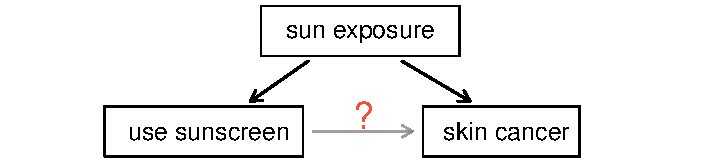
\includegraphics[width=0.57\textwidth]{ch_data_collection/figures/variables/sunCausesCancer}
\end{center}
% Some studies:
% http://www.sciencedirect.com/science/article/pii/S0140673698121682
% http://archderm.ama-assn.org/cgi/content/abstract/122/5/537
% Study with a similar scenario to that described here:
% http://onlinelibrary.wiley.com/doi/10.1002/ijc.22745/full



\begin{onebox}{Confounding variable}
A confounding variable is a variable that is associated with both the explanatory \emph{and} response variables. Because of the confounding variable's association with both variables, we do not know if the response is due to the explanatory variable or due to the confounding variable.\end{onebox}

Sun exposure is a confounding factor because it is associated with both the use of sunscreen and the development of skin cancer. People who are out in the sun all day are more likely to use sunscreen, and people who are out in the sun all day are more likely to get skin cancer. Research shows us the development of skin cancer is due to the sun exposure. The variables of sunscreen usage and sun exposure are \term{confounded}, and without this research, we would have no way of knowing which one was the true cause of skin cancer.

\begin{examplewrap}
\begin{nexample}{In a study that followed 1,169 non-diabetic men and women who had been hospitalized for a first heart attack, the people that reported eating chocolate had increased survival rate over the next 8 years than those that reported not eating chocolate.\footnotemark\, Also, those who ate more chocolate also tended to live longer on average. The researched controlled for several confounding factors, such as age, physical activity, smoking, and many other factors. Can we conclude that the consumption of chocolate caused the people to live longer?} \label{confounding_2008_chocolate_health_study}
This is an observational study, not a controlled randomized experiment. Even though the researchers controlled for many possible variables, there may still be other confounding factors. (Can you think of any that weren't mentioned?) While it is possible that the chocolate had an effect, this study cannot prove that chocolate increased the survival rate of patients.
\end{nexample}
\end{examplewrap}
\footnotetext{Janszky et al. 2009. \oiRedirect{textbook-2008_chocolate_health_study}{Chocolate consumption and mortality following a first acute myocardial infarction: the Stockholm Heart Epidemiology Program}. Journal of Internal Medicine 266:3, p248-257.} 

\begin{examplewrap}
\begin{nexample}{The authors who conducted the study did warn in the article that additional studies would be necessary to determine whether the correlation between chocolate consumption and survival translates to any causal relationship. That is, they acknowledged that there may be confounding factors. One possible confounding factor not considered was mental health. In context, explain what it would mean for mental health to be a confounding factor in this study.}
Mental health would be a confounding factor if, for example, people with better mental health tended to eat more chocolate, and those with better mental health \emph{also} were less likely to die within the 8 year study period. Notice that if better mental health were not associated with eating more chocolate, it would not be considered a confounding factor since it wouldn't explain the observed associated between eating chocolate and having a better survival rate. If better mental health were associated only with eating chocolate and not with a better survival rate, then it would also not be confounding for the same reason. Only if a variable that is associated with both the explanatory variable of interest (chocolate) and the outcome variable in the study (survival during the 8 year study period) can it be considered a confounding factor.
\end{nexample}
\end{examplewrap}

While one method to justify making causal conclusions from observational studies is to exhaust the search for confounding variables, there is no guarantee that all confounding variables can be examined or measured.

In the same way, the \data{county} data set is an observational study with confounding variables, and its data cannot be used to make causal conclusions.

\begin{exercisewrap}
\begin{nexercise}
Figure~\ref{multiunitsVsOwnership} shows a negative association between the homeownership rate and the percentage of multi-unit structures in a county. However, it is unreasonable to conclude that there is a causal relationship between the two variables. Suggest one or more other variables that might explain the relationship visible in Figure~\ref{multiunitsVsOwnership}.\footnotemark
\end{nexercise}
\end{exercisewrap}
\footnotetext{Answers will vary. Population density may be important. If a county is very dense, then this may require a larger fraction of residents to live in multi-unit structures. Additionally, the high density may contribute to increases in property value, making homeownership infeasible for many residents.}

Observational studies come in two forms: prospective and retrospective studies. A \term{prospective study} identifies individuals and collects information as events unfold. For instance, medical researchers may identify and follow a group of similar individuals over many years to assess the possible influences of behavior on cancer risk. One example of such a study is The Nurses' Health Study, started in 1976 and expanded in 1989.\footnote{\oiRedirect{textbook-channing_nurse_study}{www.channing.harvard.edu/nhs}} This prospective study recruits registered nurses and then collects data from them using questionnaires. \termsub{Retrospective studies}{retrospective studies} collect data after events have taken place, e.g. researchers may review past events in medical records. Some data sets, such as \data{county}, may contain both prospectively- and retrospectively-collected variables. Local governments prospectively collect some variables as events unfolded (e.g. retails sales) while the federal government retrospectively collected others during the 2010 census (e.g. county population counts).


%%
\subsection{Sampling from a population}

\index{sample!random sample|(}

We might try to estimate the time to graduation for Duke undergraduates in the last 5 years by collecting a sample of students. All graduates in the last 5 years represent the \emph{population}\index{population}, and graduates who are selected for review are collectively called the \emph{sample}\index{sample}. The goal is to use information from the sample to generalize or make an inference to the population.  In order to be able to generalize, we must \emph{randomly} select a sample from the population of interest. The most basic type of random selection is equivalent to how raffles are conducted. For example, in selecting graduates, we could write each graduate's name on a raffle ticket and draw 100 tickets. The selected names would represent a random sample of 100 graduates.

\begin{figure}[ht]
\centering
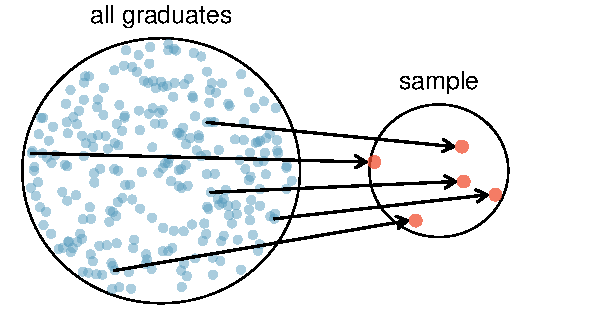
\includegraphics[width=0.47\textwidth]{ch_data_collection/figures/popToSample/popToSampleGraduates}
\caption{In this graphic, five graduates are randomly selected from the population to be included in the sample.}
\label{popToSampleGraduates}
\end{figure}

Why pick a sample randomly? Why not just pick a sample by hand? Consider the following scenario.

\D{\newpage}

\begin{examplewrap}
\begin{nexample}{Suppose we ask a student who happens to be majoring in nutrition to select several graduates for the study. What kind of students do you think she might select? Do you think her sample would be representative of all graduates?}
Perhaps she would pick a disproportionate number of graduates from health-related fields. Or perhaps her selection would be well-representative of the population. When selecting samples by hand, we run the risk of picking a \emph{biased} sample, even if that bias is unintentional or difficult to discern.
\end{nexample}
\end{examplewrap}

\begin{figure}
\centering
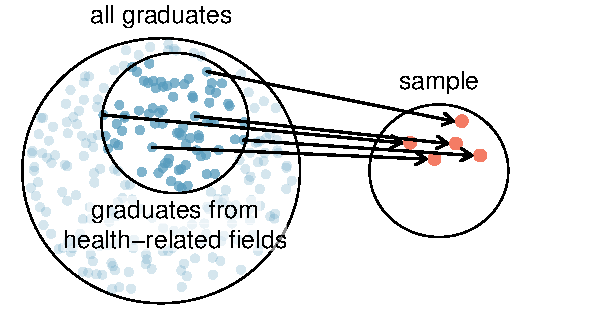
\includegraphics[width=0.47\textwidth]{ch_data_collection/figures/popToSample/popToSubSampleGraduates}
\caption{Instead of sampling from all graduates equally, a nutrition major might inadvertently pick graduates with health-related majors disproportionately often.}
\label{popToSubSampleGraduates}
\end{figure}

If the student majoring in nutrition picked a disproportionate number of graduates from health-related fields, this would introduce undercoverage bias into the sample. \termsub{Undercoverage bias}{undercoverage bias} occurs when some individuals of the population are inherently less likely to be included in the sample than others, making the sample not representative of the population.  In the example, this bias creates a problem because a degree in health-related fields might take more or less time to complete than a degree in other fields. Suppose that it takes longer. Since graduates from other fields would be less likely to be in the sample, the undercoverage bias would cause her to \emph{overestimate} the parameter.

Sampling randomly resolves the problem of undercoverage bias, \emph{if the sample is randomly selected from the entire population of interest}. If the sample is randomly selected from only a subset of the population, say, only graduates from health-related fields, then the sample will not be representative of the population of interest.  Generalizations can only be made to the population from which the sample is randomly selected.

The most basic random sample is called a \term{simple random sample}, which is equivalent to using a raffle to select cases. This means that each case in the population has an equal chance of being included and there is no implied connection between the cases in the sample.

A common downfall is a \term{convenience sample}\index{sample!convenience sample}, where individuals who are easily accessible are more likely to be included in the sample. For instance, if a political survey is done by stopping people walking in the Bronx, this will not represent all of New York City. It is often difficult to discern what sub-population a convenience sample represents.

\begin{figure}[h]
\centering
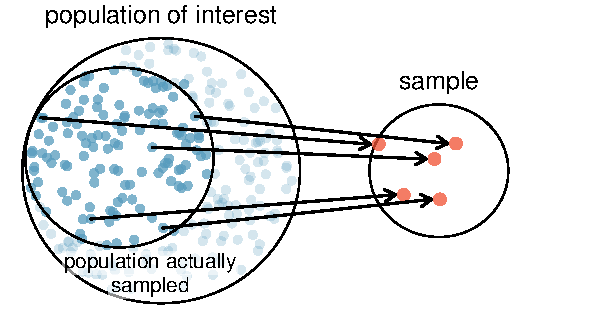
\includegraphics[width=0.5\textwidth]{ch_data_collection/figures/popToSample/surveySample}
\caption{Due to the possibility of non-response, surveys studies may only reach a certain group within the population. It is difficult, and often times impossible, to completely fix this problem.}
\label{surveySample}
\end{figure}

Similarly, a \term{volunteer sample} is one in which people's responses are solicited and those who choose to participate, respond. This is a problem because those who choose to participate may tend to have different opinions than the rest of the population, resulting in a biased sample.

\begin{exercisewrap}
\begin{nexercise}
We can easily access ratings for products, sellers, and companies through websites. These ratings are based only on those people who go out of their way to provide a rating. If 50\% of online reviews for a product are negative, do you think this means that 50\% of buyers are dissatisfied with the product?\footnotemark
\end{nexercise}
\end{exercisewrap}
\footnotetext{Answers will vary. From our own anecdotal experiences, we believe people tend to rant more about products that fell below expectations than rave about those that perform as expected. For this reason, we suspect there is a negative bias in product ratings on sites like Amazon. However, since our experiences may not be representative, we also keep an open mind.}

The act of taking a random sample helps minimize bias; however, bias can crop up in other ways. Even when people are picked at random, e.g. for surveys, caution must be exercised if the \term{non-response} \index{sample!non-response|textbf} is high. For instance, if only 30\% of the people randomly sampled for a survey actually respond, then it is unclear whether the results are \term{representative} of the entire population. This \term{non-response bias} \index{sample!non-response bias|textbf} can skew results.

Even if a sample has no undercoverage bias and no non-response bias, there is an additional type of bias that often crops up and undermines the validity of results, known as response bias. \termsub{Response bias}{response bias} refers to a broad range of factors that influence how a person responds, such as question wording, question order, and influence of the interviewer. This type of bias can be present even when we collect data from an entire population in what is called a \term{census}. Because response bias is often subtle, one must pay careful attention to how questions were asked when attempting to draw conclusions from the data.

\begin{examplewrap}
\begin{nexample}{Suppose a high school student wants to investigate the student body's opinions on the food in the cafeteria. Let's assume that she manages to survey every student in the school. How might response bias arise in this context?}
There are many possible correct answers to this question. For example, students might respond differently depending upon who asks the question, such as a school friend or someone who works in the cafeteria. The wording of the question could introduce response bias. Students would likely respond differently if asked ``Do you like the food in the cafeteria?" versus ``The food in the cafeteria is pretty bad, don't you think?"
\end{nexample}
\end{examplewrap}

\begin{onebox}{Watch out for bias}
Undercoverage bias, non-response bias, and response bias can still exist within a random sample. Always determine how a sample was chosen, ask what proportion of people failed to respond, and critically examine the wording of the questions.
\end{onebox}

When there is no bias in a sample, increasing the sample size tends to increase the precision and reliability of the estimate. When a sample is biased, it may be impossible to decipher helpful information from the data, even if the sample is very large.

\newpage 
\begin{exercisewrap}
\begin{nexercise}
A researcher sends out questionnaires to 50 randomly selected households in a particular town asking whether or not they support the addition of a traffic light in their neighborhood. Because only 20\% of the questionnaires are returned, she decides to mail questionnaires to 50 more randomly selected households in the same neighborhood. Comment on the usefulness of this approach.\footnotemark
\end{nexercise}
\end{exercisewrap}
\footnotetext{The researcher should be concerned about non-response bias, and sampling more people will not eliminate this issue. The same type of people that did not respond to the first survey are likely not going to respond to the second survey. Instead, she should make an effort to reach out to the households from the original sample that did not respond and solicit their feedback, possibly by going door-to-door.}

\index{sample!random sample|)}
\index{population|)}
\index{sample|)}




%%
\subsection[Simple, systematic, stratified, cluster, and multistage sampling]{Simple, systematic, stratified, cluster, and multistage sampling}
\label{threeSamplingMethods}

Almost all statistical methods for observational data rely on a sample being random and unbiased. When a sample is collected in a biased way, these statistical methods will not generally produce reliable information about the population.

The idea of a simple random sample was introduced in the last section. Here we provide a more technical treatment of this method and introduce four new random sampling methods: systematic, stratified, cluster, and multistage.\footnote{Multistage sampling is not part of the AP syllabus.} Figure~\ref{simple_systematic} provides a graphical representation of simple versus systematic sampling while Figure~\ref{stratified_cluster_multistage} provides a graphical representation of stratified, cluster, and multistage sampling.


\begin{figure}[p]
\centering
\Figures{0.9}{samplingMethodsFigure}{simple_systematic}
\caption{Examples of simple random sampling and systematic sampling. In the top panel, simple random sampling was used to randomly select 18 cases. In the lower panel, systematic random sampling was used to select every 7th individual.}
\label{simple_systematic}
\end{figure}

\termsub{Simple random sampling}{sample!simple random sampling} is probably the most intuitive form of random sampling. Consider the salaries of Major League Baseball (MLB) players, where each player is a member of one of the league's 30 teams. For the 2019 season, N, the population size or total number of players, is 750. To take a simple random sample of \textit{n} = 120 of these baseball players and their salaries, we could number each player from 1 to 750. Then we could randomly select 120 numbers between 1 and 750 (without replacement) using a random number generator or random digit table. The players with the selected numbers would comprise our sample.

Two properties are always true in a simple random sample:
\begin{enumerate}
\item Each case in the population has an equal chance of being included in the sample.
\item Each \emph{group} of \textit{n} cases has an equal chance of making up the sample.
\end{enumerate}

The statistical methods in this book focus on data collected using simple random sampling. Note that Property 2 -- that each group of \textit{n} cases has an equal chance making up the sample -- is not true for the remaining four sampling techniques. As you read each one, consider why.

Though less common than simple random sampling, \termsub{systematic sampling}{sample!systematic sampling} is sometimes used when there exists a convenient list of all of the individuals of the population. Suppose we have a roster with the names of all the MLB players from the 2019 season. To take a systematic random sample, number them from 1 to 750. Select one random number between 1 and 750 and let that player be the first individual in the sample. Then, depending on the desired sample size, select every 10th number or 20th number, for example, to arrive at the sample.\footnote{If we want a sample of size \textit{n} = 150, it would make sense to select every 5th player since \mbox{$750/150 = 5$.} Suppose we randomly select the number 741. Then player 741, 746, 1, 6, 11, $\cdots$ , 731, and 736 would make up the sample.} If there are no patterns in the salaries based on the numbering then this could be a reasonable method.

\begin{examplewrap}
\begin{nexample}{A systematic sample is not the same as a simple random sample. Provide an example of a sample that can come from a simple random sample but not from a systematic random sample.}
Answers can vary. If we take a sample of size 3, then it is possible that we could sample players numbered 1, 2, and 3 in a simple random sample. Such a sample would be impossible from a systematic sample. Property~2 of simple random samples does not hold for other types of random samples.
\end{nexample}
\end{examplewrap}

\D{\newpage}

Sometimes there is a variable that is known to be associated with the quantity we want to estimate. In this case, a stratified random sample might be selected. \termsub{Stratified sampling}{sample!stratified sampling} is a divide-and-conquer sampling strategy. The population is divided into groups called \term{strata}\index{sample!strata|textbf}. The strata are chosen so that similar cases are grouped together and a sampling method, usually simple random sampling, is employed to select a certain number or a certain proportion of the whole within each stratum. In the baseball salary example, the 30 teams could represent the strata; some teams have a lot more money (we're looking at you, Yankees).

\begin{figure}
\centering
\Figures{0.85}{samplingMethodsFigure}{stratified_cluster_multistage}
\caption{Examples of stratified, cluster, and multistage sampling. In the top panel, stratified sampling was used: cases were grouped into strata, and then simple random sampling was employed within each stratum. In the middle panel, cluster sampling was used, where data were binned into nine cluster and three clusters were randomly selected. In the bottom panel, multistage sampling was used. Data were binned into the nine clusters, three of the cluster were randomly selected, and then six cases were randomly sampled in each of the three selected clusters.}
\label{stratified_cluster_multistage}
\end{figure}

\begin{examplewrap}
\begin{nexample}{For this baseball example, briefly explain how to select a stratified random sample of size \textit{n} = 120. }
Each team can serve as a stratum, and we could take a simple random sample of 4 players from each of the 30 teams, yielding a sample of 120 players.
\end{nexample}
\end{examplewrap}

Stratified sampling is inherently different than simple random sampling. For example, the stratified sampling approach described would make it impossible for the entire Yankees team to be included in the sample.

\begin{examplewrap}
\begin{nexample}{Stratified sampling is especially useful when the cases in each stratum are very similar \emph{with respect to the outcome of interest}. Why is it good for cases within each stratum to be very similar?}
We should get a more stable estimate for the subpopulation in a stratum if the cases are very similar. These improved estimates for each subpopulation will help us build a reliable estimate for the full population. For example, in a simple random sample, it is possible that just by random chance we could end up with proportionally too many Yankees players in our sample, thus overestimating the true average salary of all MLB players. A stratified random sample can assure proportional representation from each team.
\end{nexample}
\end{examplewrap}

Next, let's consider a sampling technique that randomly selects groups of people. \termsub{Cluster sampling}{sample!cluster sampling} is much like simple random sampling, but instead of randomly selecting \emph{individuals}, we randomly select groups or \term{clusters}. Unlike stratified sampling, cluster sampling is most helpful when there is a lot of case-to-case variability within a cluster but the clusters themselves don't look very different from one another. That~is, we expect individual strata to be \term{homogeneous} (self-similar), while we expect individual clusters to be \term{heterogeneous} (diverse) with respect to the variable of interest.  

Sometimes cluster sampling can be a more economical random sampling technique than the alternatives. For example, if neighborhoods represented clusters, this sampling method works best when each neighborhood is very diverse. Because each neighborhood itself encompasses diversity, a cluster sample can reduce the time and cost associated with data collection, because the interviewer would need only go to some of the neighborhoods rather than to all parts of a city, in order to collect a useful sample.

\termsub{Multistage sampling}{sample!multistage sampling}, also called \termsub{multistage cluster sampling}{sample!multistage cluster sampling}, is a two (or more) step strategy. The first step is to take a cluster sample, as described above. Then, instead of including all of the individuals in these clusters in our sample, a second sampling method, usually simple random sampling, is employed within each of the selected clusters. In the neighborhood example, we could first randomly select some number of neighborhoods and then take a simple random sample from just those selected neighborhoods. As seen in Figure~\ref{stratified_cluster_multistage}, stratified sampling requires observations to be sampled from \emph{every} stratum. Multistage sampling selects observations \emph{only} from those clusters that were randomly selected in the first step.

It is also possible to have more than two steps in multistage sampling. Each cluster may be naturally divided into subclusters. For example, each neighborhood could be divided into streets. To take a three-stage sample, we could first select some number of clusters (neighborhoods), and then, within the selected clusters, select some number of subclusters (streets). Finally, we could select some number of individuals from each of the selected streets.

\begin{examplewrap}
\begin{nexample}{Suppose we are interested in estimating the proportion of students at a certain school that have part-time jobs. It is believed that older students are more likely to work than younger students. What sampling method should be employed? Describe how to collect such a sample to get a sample size of 60.}
Because grade level affects the likelihood of having a part-time job, we should take a stratified random sample. To do this, we can take a simple random sample of 15 students from each grade. This will give us equal representation from each grade. Note: in a simple random sample, just by random chance we might get too many students who are older or younger, which could make the estimate too high or too low. Also, there are no well-defined clusters in this example. We~wouldn't want to use the grades as clusters and sample everyone from a couple of the grades. This would create too large a sample and would not give us the nice representation from each grade afforded by the stratified random sample.
\end{nexample}
\end{examplewrap}

\begin{examplewrap}
\begin{nexample}{Suppose we are interested in estimating the malaria rate in a densely tropical portion of rural Indonesia. We learn that there are 30 villages in that part of the Indonesian jungle, each more or less similar to the next. Our goal is to test 150 individuals for malaria. What sampling method should be employed?}
A simple random sample would likely draw individuals from all 30 villages, which could make data collection extremely expensive. Stratified sampling would be a challenge since it is unclear how we would build strata of similar individuals. However, multistage cluster sampling seems like a very good idea. First, we might randomly select half the villages, then randomly select 10 people from each. This would probably reduce our data collection costs substantially in comparison to a simple random sample and would still give us reliable information.
\end{nexample}
\end{examplewrap}

\begin{onebox}{Advanced sampling techniques require advanced methods}
{The methods of inference covered in this book generally only apply to simple random samples. More advanced analysis techniques are required for systematic, stratified, cluster, and multistage random sampling.}
\end{onebox}


\D{\newpage}

%%
\subsection*{Section summary}

\begin{itemize}
\item In an \term{observational study}, one must always consider the existence of \termsub{confounding factors}{confounding factor}.  A confounding factor is a ``spoiler variable" that could explain an observed relationship between the explanatory variable and the response.  Remember:  For a variable to be confounding it must be associated with both the explanatory variable \textit{and} the response variable.

\item When taking a sample from a population, avoid \termsub{convenience samples}{convenience sample} and \termsub{volunteer samples}{volunteer sample}, which likely introduce bias.  Instead, use a \term{random} sampling method.

\item Generalizations from a sample can be made to a population only if the sample is random.  Furthermore, the generalization can be made only to the population from which the sample was randomly selected, not to a larger or different population.  

\item Random sampling from the entire population of interest avoids the problem of \term{undercoverage bias}.  However, \term{response bias} and \term{non-response} bias can be present in any type of sample, random or not.

\item In a \term{simple random sample}, every \textit{individual} as well as every \textit{group of individuals} has the same probability of being in the sample.  A common way to select a simple random sample is to number each individual of the population from 1 to N.  Using a random digit table or a random number generator, numbers are randomly selected without replacement and the corresponding individuals become part of the sample.

\item A \term{systematic random sample} involves choosing from of a population using a random starting point, and then selecting members according to a fixed, periodic interval (such as every 10th member). 

\item A \term{stratified random sample} involves randomly sampling from \textit{every} \term{strata}, where the strata should correspond to a variable thought to be associated with the variable of interest.  This ensures that the sample will have appropriate representation from each of the different strata and reduces variability in the sample estimates.

\item A \term{cluster random sample} involves randomly selecting a set of \term{clusters}, or groups, and then collecting data on all individuals in the selected clusters. This can be useful when sampling clusters is more convenient and less expensive than sampling individuals, and it is an effective strategy when each cluster is approximately representative of the population.  

\item Remember:  \textit{Individual strata should be homogeneous (self-similar), while individual clusters should be heterogeneous (diverse)}.  For example, if smoking is correlated with what is being estimated, let one stratum be all smokers and the other be all non-smokers, then randomly select an appropriate number of \textit{individuals} from \textit{each} strata.  Alternately, if age is correlated with the variable being estimated, one could randomly select a \textit{subset} of clusters, where each cluster has mixed age groups.


\end{itemize}

%%%section exercises
{\exercisesheader{}
% 19

\eoce{\qt{Course satisfaction across sections\label{course_satisfaction_sections}} 
A large college class has 160 students. All 160 students attend the lectures 
together, but the students are divided into 4 groups, each of 40 students, 
for lab sections administered by different teaching assistants. The professor 
wants to conduct a survey about how satisfied the students are with the course, 
and he believes that the lab section a student is in might affect the student's 
overall satisfaction with the course.
\begin{parts}
\item What type of study is this?
\item Suggest a sampling strategy for carrying out this study.
\end{parts}
}{}

% 20

\eoce{\qt{Housing proposal across dorms\label{housing_proposal_dorms}} On a large 
college campus first-year students and sophomores live in dorms located on 
the eastern part of the campus and juniors and seniors live in dorms located 
on the western part of the campus. Suppose you want to collect student opinions 
on a new housing structure the college administration is proposing and you want 
to make sure your survey equally represents opinions from students from all years.
\begin{parts}
\item What type of study is this?
\item Suggest a sampling strategy for carrying out this study.
\end{parts}
}{}

% 21

\eoce{\qt{Internet use and life expectancy\label{internet_life_expectancy}} The 
following scatterplot was created as part of a study evaluating the 
relationship between estimated life expectancy at birth (as of 2014) and 
percentage of internet users (as of 2009) in 208 countries for which such 
data were available.\footfullcite{data:ciaFactbook}

\noindent\begin{minipage}[c]{0.44\textwidth}
\begin{parts}
\item Describe the relationship between life expectancy and percentage of 
internet users.
\item What type of study is this?
\item State a possible confounding variable that might explain this relationship 
and describe its potential effect.
\end{parts} \vspace{15mm}
\end{minipage}
\begin{minipage}[r]{0.55\textwidth}
\href{\oiRedirectUrl{tableau-scatter-lifeexp-internetusers}}{
\hfill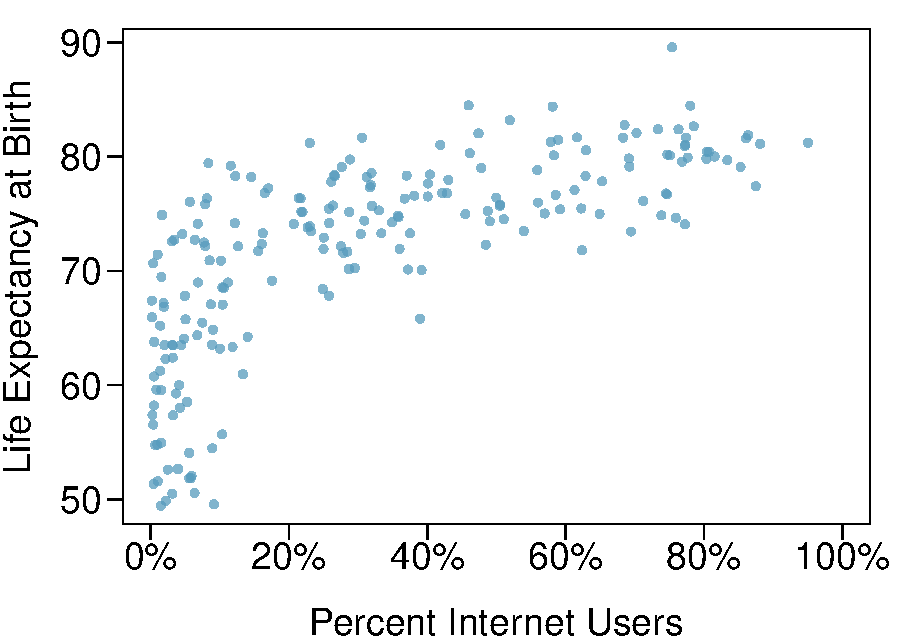
\includegraphics[width = 0.87\textwidth]{ch_data_collection/figures/eoce/internet_life_expectancy/internet_life_expectancy}
}
\tableauhref{tableau-scatter-lifeexp-internetusers}

\end{minipage}

}{}

% 22

\eoce{\qt{Stressed out, Part I\label{stressed_out_observational}} A study that 
surveyed a random sample of otherwise healthy high school students found that 
they are more likely to get muscle cramps when they are stressed. The study 
also noted that students drink more coffee and sleep less when they are 
stressed.
\begin{parts}
\item What type of study is this?
\item Can this study be used to conclude a causal relationship between 
increased stress and muscle cramps?
\item State possible confounding variables that might explain the observed 
relationship between increased stress and muscle cramps. 
\end{parts}
}{}

% 23

\eoce{\qt{Evaluate sampling methods\label{evaluate_sampling_methods}} A university wants to 
determine what fraction of its undergraduate student body support a new \$25 annual fee 
to improve the student union. For each proposed method below, indicate whether 
the method is reasonable or not.
\begin{parts}
\item Survey a simple random sample of 500 students.
\item Stratify students by their field of study, then sample 10\% of students from  
each stratum.
\item Cluster students by their ages (e.g. 18 years old in one cluster, 19 years 
old in one cluster, etc.), then randomly sample three clusters and survey all 
students in those clusters.
\end{parts}
}{}

% 24

\eoce{\qt{Random digit dialing\label{random_digit_dialing}} The Gallup Poll uses a 
procedure called random digit dialing, which creates phone numbers based on 
a list of all area codes in America in conjunction with the associated number 
of residential households in each area code. Give a possible reason the Gallup 
Poll chooses to use random digit dialing instead of picking phone numbers 
from the phone book.
}{}

\D{\newpage}

% 25

\eoce{\qt{Haters are gonna hate, study confirms\label{scope_haters}} A study 
published in the \textit{Journal of Personality and Social Psychology} asked a 
group of 200 randomly sampled men and women to evaluate how they felt about 
various subjects, such as camping, health care, architecture, taxidermy, 
crossword puzzles, and Japan in order to measure their dispositional attitude 
towards mostly independent stimuli. Then, they presented the participants with 
information about a new product: a microwave oven. This microwave oven does 
not exist, but the participants didn't know this, and were given three 
positive and three negative fake reviews. People who reacted positively to the 
subjects on the dispositional attitude measurement also tended to react 
positively to the microwave oven, and those who reacted negatively also tended 
to react negatively to it. Researchers concluded that ``some people tend to 
like things, whereas others tend to dislike things, and a more thorough 
understanding of this tendency will lead to a more thorough understanding of 
the psychology of attitudes." \footfullcite{Hepler:2013}
\begin{parts}
\item What are the cases?
\item What is (are) the response variable(s) in this study?
\item What is (are) the explanatory variable(s) in this study?
\item Does the study employ random sampling?
\item Is this an observational study or an experiment? Explain your reasoning.
\item Can we establish a causal link between the explanatory and response 
variables?
\item Can the results of the study be generalized to the population at large?
\end{parts}
}{}

% 26

\eoce{\qt{Family size\label{family_size}} Suppose we want to estimate household 
size, where a ``household" is defined as people living together in the 
same dwelling, and sharing living accommodations. If we select students 
at random at an elementary school and ask them what their family size is, 
will this be a good measure of household size? Or will our average be 
biased? If so, will it overestimate or underestimate the true value?
}{}

% 27

\eoce{\qt{Sampling strategies\label{sampling_strategies}} A statistics student who is curious about the relationship between the amount of time students spend on social networking sites and their performance at school decides to conduct a survey. Various research strategies for collecting data are described below. In each, name the sampling method proposed and any bias you might expect.
\begin{parts}
\item He randomly samples 40 students from the study's population, gives them the survey, asks them to fill it out and bring it back the next day.
\item He gives out the survey only to his friends, making sure each one of them fills out the survey.
\item He posts a link to an online survey on Facebook and asks his friends to fill out the survey.
\item He randomly samples 5 classes and asks a random sample of students from those classes to fill out the survey.
\end{parts}
}{}

% 28

\eoce{\qt{Reading the paper\label{reading_paper}} Below are excerpts from two 
articles published in the \emph{NY Times}:
\begin{parts}
\item An article titled \emph{Risks: Smokers Found More Prone to Dementia} 
states the following: \footfullcite{news:smokingDementia}
\begin{adjustwidth}{1em}{1em}
{\footnotesize ``Researchers analyzed data from 23,123 health plan members who 
participated in a voluntary exam and health behavior survey from 1978 to 1985, 
when they were 50-60 years old. 23 years later, about 25\% of the group had 
dementia, including 1,136 with Alzheimer's disease and 416 with vascular 
dementia. After adjusting for other factors, the researchers concluded that 
pack-a-day smokers were 37\% more likely than nonsmokers to develop dementia, 
and the risks went up with increased smoking; 44\% for one to two packs a day; 
and twice the risk for more than two packs."}
\end{adjustwidth}
Based on this study, can we conclude that smoking causes dementia later in 
life? Explain your reasoning.
\item Another article titled \emph{The School Bully Is Sleepy} states the 
following: \footfullcite{news:bullySleep}
\begin{adjustwidth}{1em}{1em}
{\footnotesize ``The University of Michigan study, collected survey data from 
parents on each child's sleep habits and asked both parents and teachers to 
assess behavioral concerns. About a third of the students studied were 
identified by parents or teachers as having problems with disruptive behavior 
or bullying. The researchers found that children who had behavioral issues and 
those who were identified as bullies were twice as likely to have shown 
symptoms of sleep disorders."}
\end{adjustwidth}
A friend of yours who read the article says, ``The study shows that sleep 
disorders lead to bullying in school children." Is this statement justified? 
If not, how best can you describe the conclusion that can be drawn from this 
study?
\end{parts}
}{}
}


%_____________________________________
\section[Experiments]{Experiments }
\label{experimentsSection}
\sectionintro{
\noindent%
You would like to determine if drinking a cup of tea each morning will cause students to perform better on tests.
What are different ways you could design an experiment to answer this question?
What are possible sources of bias, and how would you try to minimize them?
The goal of an experiment is to be able to draw a causal conclusion about the effect of a treatment -- in this case, drinking tea.
If the design is poor, a causal conclusion cannot be drawn, even if you observe an association between drinking tea and performing better on tests.
This is why it is crucial to start with a well-designed experiment.


\subsection*{Learning objectives}
\begin{enumerate}
\setlength{\itemsep}{0mm}
\item Identify the subjects/experimental units, treatments, and response variable in an experiment. 
 
\item Identify the three main principles of experiment design and explain their purpose: direct control, randomization, and replication.
 
\item Explain placebo effect and describe when and how to implement a single-blind and a double-blind experiment.
 
\item Identify and describe how to implement the following three experimental designs: completely randomized design, blocked design, and matched pairs design.
 
\item Explain the purpose of random assignment or randomization in each of the three experimental designs.
 
\item Explain how to randomize treatments in a completely randomized design using technology or a table of random digits (make sure this is explained).
 
\item Explain when it is reasonable to draw a causal conclusion about the effect of a treatment.
 
\item  Identify the number of factors in experiment, the number of levels for each factor and the total number of treatments.

\end{enumerate}
}

%%
\subsection{Reducing bias in human experiments}
\label{biasInHumanExperiments}

In the last section we investigated observational studies and sampling strategies. While these are effective tools for answering certain research questions, often times researchers want to measure the effect of a treatment. In this case, they must carry out an experiment. Just as randomization is essential in sampling in order to avoid selection bias, randomization is essential in the context of experiments to determine which subjects will receive which treatments. If the researcher chooses which patients are in the treatment and control groups, she may unintentionally place sicker patients in the treatment group, biasing the experiment against the treatment.

Randomized experiments are essential for investigating cause and effect relationships, but they do not ensure an unbiased perspective in all cases. Human studies are perfect examples where bias can unintentionally arise. Here we reconsider a study where a new drug was used to treat heart attack patients.\footnote{Anturane Reinfarction Trial Research Group. 1980. Sulfinpyrazone in the prevention of sudden death after myocardial infarction. New England Journal of Medicine 302(5):250-256.} In particular, researchers wanted to know if the drug reduced deaths in patients.

These researchers designed a randomized experiment because they wanted to draw causal conclusions about the drug's effect. Study volunteers\footnote{Human subjects are often called \term{patients}, \term{volunteers}, or \term{study participants}.} were randomly placed into two study groups. One group, the \term{treatment group}, received the drug. The other group, called the \term{control group}, did not receive any drug treatment. In an experiment, the explanatory variable is also called a \term{factor}. Here the factor is receiving the drug treatment. It has two \term{levels}: yes and no, thus it is categorical. The response variable is whether or not patients died within the time frame of the study. It is also categorical.

Put yourself in the place of a person in the study. If you are in the treatment group, you are given a fancy new drug that you anticipate will help you. On the other hand, a person in the other group doesn't receive the drug and sits idly, hoping her participation doesn't increase her risk of death. These perspectives suggest there are actually two effects: the one of interest is the effectiveness of the drug, and the second is an emotional effect that is difficult to quantify.

Researchers aren't usually interested in the emotional effect, which might bias the study. To circumvent this problem, researchers do not want patients to know which group they are in. When researchers keep the patients uninformed about their treatment, the study is said to be \term{blind} or \term{single-blind}. But there is one problem: if a patient doesn't receive a treatment, she will know she is in the control group. The solution to this problem is to give fake treatments to patients in the control group. A fake treatment is called a \term{placebo}, and an effective placebo is the key to making a study truly blind. A classic example of a placebo is a sugar pill that is made to look like the actual treatment pill. Often times, a placebo results in a slight but real improvement in patients. This effect has been dubbed the \term{placebo~effect}.

The patients are not the only ones who should be blinded: doctors and researchers can accidentally bias a study. When a doctor knows a patient has been given the real treatment, she might inadvertently give that patient more attention or care than a patient that she knows is on the placebo. To guard against this bias, which again has been found to have a measurable effect in some instances, most modern studies employ a \term{double-blind} setup where researchers who interact with subjects and are responsible for measuring the response variable are, just like the subjects, unaware of who is or is not receiving the treatment.\footnote{There are always some researchers involved in the study who do know which patients are receiving which treatment. However, they do not interact with the study's patients and do not tell the blinded health care professionals who is receiving which treatment.}


\begin{exercisewrap}
\begin{nexercise}
Look back to the study in Section~\ref{basicExampleOfStentsAndStrokes} where researchers were testing whether stents were effective at reducing strokes in at-risk patients. Is this an experiment? Was the study blinded? Was it double-blinded?\footnotemark
\end{nexercise}
\end{exercisewrap}
\footnotetext{The researchers assigned the patients into their treatment groups, so this study was an experiment. However, the patients could distinguish what treatment they received, so this study was not blind. The study could not be double-blind since it was not blind.}



%\D{\newpage}

%%
\subsection{Principles of experimental design}
\label{experimentalDesignPrinciples}

\noindent Well-conducted experiments are built on three main principles.

\begin{description}
\setlength{\itemsep}{0mm}
\item[\termsub{Direct Control.}{direct control}] Researchers assign treatments to cases, and they do their best to \term{control} any other differences in the groups. They want the groups to be as identical as possible \emph{except for the treatment}, so that at the end of the experiment any difference in response between the groups can be attributed to the treatment and not to some other confounding or lurking variable. For example, when patients take a drug in pill form, some patients take the pill with only a sip of water while others may have it with an entire glass of water. To control for the effect of water consumption, a doctor may ask all patients to drink a 12 ounce glass of water with the pill.

Direct control refers to variables that the researcher can control, or make the same. A researcher can directly control the appearance of the treatment, the time of day it is taken, etc. She cannot directly control variables such as gender or age. To control for these other types of variables, she might consider blocking, which is described in Section~\ref{CompletelyRandomizedBlockedAndMatchedPairsDesign}.

\item[Randomization.] Researchers randomize patients into treatment groups to account for variables that cannot be controlled. For example, some patients may be more susceptible to a disease than others due to their dietary habits. Randomizing patients into the treatment or control group helps \emph{even out} the effects of such differences, and it also prevents accidental bias from entering the study.

\item[Replication.] The more cases researchers observe, the more accurately they can estimate the effect of the explanatory variable on the response. In an experiment with six subjects, even if there is randomization, it is quite possible for the three healthiest people to be in the same treatment group. In a randomized experiment with 100 people, it is virtually impossible for the healthiest 50 people to end up in the same treatment group. In a single study, we \term{replicate} by imposing the treatment on a sufficiently large number of subjects or experimental units. A group of scientists may also replicate an entire study to verify an earlier finding. However, each study should ensure a sufficiently large number of subjects because, in many cases, there is no opportunity or funding to carry out the entire experiment again.
\end{description}

It is important to incorporate these design principles into any experiment. If they are lacking, the inference methods presented in the following chapters will not be applicable and their results may not be trustworthy. In the next section we will consider three types of experimental design.


%%
\subsection{Completely randomized, blocked, and matched pairs design}
\label{CompletelyRandomizedBlockedAndMatchedPairsDesign}

\index{completely randomized experiment|(}
\index{blocked experiment|(}
\index{matched pairs|(}

A \term{completely randomized experiment} is one in which the subjects or experimental units are randomly assigned to each group in the experiment. Suppose we have three treatments, one of which may be a placebo, and 300 subjects. To carry out a completely randomized design, we could randomly assign each subject a unique number from 1 to 300, then subjects with numbers 1-100 would get treatment~1, subjects 101-200 would get treatment~2, and subjects 201- 300 would get treatment~3. Note that this method of randomly allocating subjects to treatments in not equivalent to taking a simple random sample. Here we are not sampling a subset of a population; we are randomly \emph{splitting} subjects into groups.

% ZZQ - The following two paragraphs have an awkward transition.

While it might be ideal for the subjects to be a random sample of the population of interest, that is rarely the case. Subjects must volunteer to be part of an experiment. However, because randomization is incorporated in the splitting of the groups, we can still use statistical techniques to check for a causal connection, though the precise population for which the conclusion applies may be unclear. For example, if an experiment to determine the most effective means to encourage individuals to vote is carried out only on college students, we may not be able to generalize the conclusions of the experiment to all adults in the population.

\begin{figure}
\centering
\Figure{0.78}{figureShowingBlocking}
\caption{Blocking using a variable depicting patient risk. Patients are first divided into low-risk and high-risk blocks, then each block is evenly separated into the treatment groups using randomization. This strategy ensures an equal representation of patients in each treatment group from both the low-risk and high-risk categories.}
\label{figureShowingBlocking}
\end{figure}

Researchers sometimes know or suspect that another variable, other than the treatment, influences the response. Under these circumstances, they may carry out a \term{blocked experiment}. In this design, they first group individuals into \term{blocks} based on the identified variable and then randomize subjects within each block to the treatment groups. This strategy is referred to as \term{blocking}. For instance, if we are looking at the effect of a drug on heart attacks, we might first split patients in the study into low-risk and high-risk blocks. Then we can randomly assign half the patients from each block to the control group and the other half to the treatment group, as shown in Figure~\ref{figureShowingBlocking}. At the end of the experiment, we would incorporate this blocking into the analysis. By blocking by risk of patient, we control for this possible confounding factor. Additionally, by randomizing subjects to treatments within each block, we attempt to even out the effect of variables that we cannot block or directly control.

\begin{examplewrap}
\begin{nexample}{An experiment will be conducted to compare the effectiveness of two methods for quitting smoking. Identify a variable that the researcher might wish to use for blocking and describe how she would carry out a blocked experiment.}
The researcher should choose the variable that is most likely to influence the response variable - whether or not a smoker will quit. A reasonable variable, therefore, would be the number of years that the smoker has been smoking. The subjects could be separated into three blocks based on number of years of smoking and each block randomly divided into the two treatment groups.
\end{nexample}
\end{examplewrap}

Even in a blocked experiment with randomization, other variables that affect the response can be distributed unevenly among the treatment groups, thus biasing the experiment in one direction. A third type of design, known as \term{matched pairs} addresses this problem. In a matched pairs experiment, pairs of people are matched on as many variables as possible, so that the comparison happens between very similar cases. This is actually a special type of blocked experiment, where the blocks are of size two.

An alternate form of matched pairs involves each subject receiving \emph{both} treatments. Randomization can be incorporated by randomly selecting half the subjects to receive treatment 1 first, followed by treatment 2, while the other half receives treatment 2 first, followed by treatment.

\begin{exercisewrap}
\begin{nexercise}
How and why should randomization be incorporated into a matched pairs design?\footnotemark
\end{nexercise}
\end{exercisewrap}
\footnotetext{Assume that all subjects received treatment 1 first, followed by treatment 2. If the variable being measured happens to increase naturally over the course of time, it would appear as though treatment 2 had a greater effect than it really did.} 

%\Add{This type of matched pairs design is optimal, because it allows us to compare each subject to herself, rather than comparing a group of subjects to a separate group of subjects. By doing this, we control for the inherent variability in response from person to person.} % This is not necessarily true: treatments can interact in unexpected ways, even if given over long periods of time. Even in the lotion example, handedness might be more important in some situations, e.g. if looking at how much lotion rubs off. Careful matched individuals might be a better design in that situation.

\begin{exercisewrap}
\begin{nexercise}
Matched pairs sometimes involves each subject receiving both treatments at the same time. For example, if a hand lotion was being tested, half of the subjects could be randomly assigned to put Lotion A on the left hand and Lotion B on the right hand, while the other half of the subjects would put Lotion B on the left hand and Lotion A on the right hand. Why would this be a better design than a completely randomized experiment in which half of the subjects put Lotion A on both hands and the other half put Lotion B on both hands?\footnotemark\end{nexercise}
\end{exercisewrap}
\footnotetext{The dryness of people's skins varies from person to person, but probably less so from one person's right hand to left hand. With the matched pairs design, we are able control for this variability by comparing each person's right hand to her left hand, rather than comparing some people's hands to other people's hands (as you would in a completely randomized experiment).} % In a completely randomized experiment, it is possible that one group, just by chance, could have more people with especially dry skin, thus biasing the results against the lotion that they used.} % Cutting for brevity.

Because it is essential to identify the type of data collection method used when choosing an appropriate inference procedure, we will revisit sampling techniques and experiment design in the subsequent chapters on inference.

\index{matched pairs|)}
\index{blocked experiment|)}
\index{completely randomized experiment|)}


\D{\newpage}

%%
\subsection{Testing more than one variable at a time}

Some experiments study more than one factor (explanatory variable) at a time, and each of these factors may have two or more levels (possible values). For example, suppose a researcher plans to investigate how the type and volume of music affect a person's performance on a particular video game. Because these two factors, \var{type} and \var{volume}, could interact in interesting ways, we do not want to test one factor at a time. %
%Instead, we want to do a \term{factorial experiment} in which 
Instead, we want to do an experiment in which
we test all the \emph{combinations} of the factors. Let's say that \var{volume} has two levels (soft and loud) and that \var{type} has three levels (dance, classical, and punk). Then, we would want to carry out the experiment at each of the six (2 x 3 = 6) combinations: soft dance, soft classical, soft punk, loud dance, loud classical, loud punk. Each of the these combinations is a \term{treatment}. Therefore, this experiment will have 2 factors and 6 treatments. In order to replicate each treatment 10 times, one would need to play the game 60 times.

\begin{exercisewrap}
\begin{nexercise}A researcher wants to compare the effectiveness of four different drugs. She also wants to test each of the drugs at two doses: low and high. Describe the factors, levels, and treatments of this experiment.\footnotemark
\end{nexercise}
\end{exercisewrap}
\footnotetext{There are two factors: type of drug, which has four levels, and dose, which has 2 levels. There will be 4 x 2 = 8 treatments: drug 1 at low dose, drug 1 at high dose, drug 2 at low dose, and so on.}

As the number of factors and levels increases, the number of treatments become large and the analysis of the resulting data becomes more complex, requiring the use of advanced statistical methods. We will investigate only one factor at a time in this book.


\D{\newpage}

%%
\subsection*{Section summary}

\begin{itemize}
\item In an \term{experiment}, researchers impose a \term{treatment} to test its effects.  In order for observed differences in the response to be attributed to the treatment and not to some other factor, it is important to make the treatment groups and the conditions for the treatment groups as similar as possible.

\item Researchers use \term{direct control}, ensuring that variables that are within their power to modify (such as drug dosage or testing conditions) are made the \textit{same} for each treatment group.  

\item Researchers \term{randomly} assign subjects to the treatment groups so that the effects of uncontrolled and potentially confounding variables are \textit{evened out} among the treatment groups.

\item \termsub{Replication}{replication}, or imposing the treatments on many subjects, gives more data and decreases the likelihood that the treatment groups differ on some characteristic due to chance alone (i.e. in spite of the randomization).  

\item An ideal experiment is \term{randomized}, \termsub{controlled}{control}, and \term{double-blind}.  

\item A \term{completely randomized experiment} involves randomly assigning the subjects to the different treatment groups.  To do this, first number the subjects from 1 to N.  Then, randomly choose some of those numbers and assign the corresponding subjects to a treatment group.  Do this in such a way that the treatment group sizes are balanced, unless there exists a good reason to make one treatment group larger than another.

\item In a \term {blocked experiment}, subjects are first separated by a variable thought to affect the response variable.  Then, within \textit{each} block, subjects are randomly assigned to the treatment groups as described above, allowing the researcher to compare like to like within each block. 

\item When feasible, a \term{matched-pairs experiment} is ideal, because it allows for the best comparison of like to like.  A matched-pairs experiment can be carried out on pairs of subjects that are meaningfully paired, such as twins, or it can involve all subjects receiving both treatments, allowing subjects to be compared to \textit{themselves}.  

\item A treatment is also called a \term{factor} or explanatory variable.  Each treatment/factor can have multiple \term{levels}, such as yes/no or low/medium/high.  When an experiment includes many factors, multiplying the number of levels of the factors together gives the total number of treatment groups.  

\item In an experiment, blocking, randomization, and direct control are used to \textit{control for confounding factors}.

\end{itemize}


%%%section exercises
{\exercisesheader{}

% 29 - light_exam_performance

\eoce{\qt{Light and exam performance\label{light_exam_performance}} A study is designed to 
test the effect of light level on exam performance of students. The researcher believes 
that light levels might have different effects on males and females, so wants to make 
sure both are equally represented in each treatment. The treatments are fluorescent 
overhead lighting, yellow overhead lighting, no overhead lighting (only desk lamps). 
\begin{parts}
\item What is the response variable?
\item What is the explanatory variable? What are its levels?
\item What is the blocking variable? What are its levels?
\end{parts}
}{}

% 30 - vitamin_supplement

\eoce{\qt{Vitamin supplements\label{vitamin_supplement}}
To assess the effectiveness of taking large doses
of vitamin C in reducing the duration of the common cold, 
researchers recruited 400 healthy volunteers from staff
and students at a university.
A~quarter of the patients were assigned a placebo,
and the rest were evenly divided between 1g Vitamin C,
3g Vitamin C, or 3g Vitamin C plus additives to be
taken at onset of a cold for the following two days.
All tablets had identical appearance and packaging.
The nurses who handed the prescribed pills to the
patients knew which patient received which treatment,
but the researchers assessing the patients when they
were sick did not. 
No significant differences were observed in any measure
of cold duration or severity between the four groups,
and the placebo group had the shortest duration of 
symptoms.\footfullcite{Audera:2001}
\begin{parts}
\item Was this an experiment or an observational study? Why?
\item What are the explanatory and response variables in this study?
\item Were the patients blinded to their treatment?
\item Was this study double-blind?
\item Participants are ultimately able to choose whether or not to use the pills 
prescribed to them. We might expect that not all of them will adhere and take their 
pills. Does this introduce a confounding variable to the study? Explain your reasoning.
\end{parts}
}{}

% 31 - light_noise_exam_performance

\eoce{\qt{Light, noise, and exam performance\label{light_noise_exam_performance}} A study is 
designed to test the effect of light level and noise level on exam performance of 
students. The researcher believes that light and noise levels might have different 
effects on males and females, so wants to make sure both are equally represented in each 
treatment. The light treatments considered are fluorescent overhead lighting, yellow 
overhead lighting, no overhead lighting (only desk lamps). The noise treatments 
considered are no noise,  construction noise, and human chatter noise.
\begin{parts}
\item What type of study is this?
\item How many factors are considered in this study? Identify them, and describe their 
levels.
\item What is the role of the sex variable in this study?
\end{parts}
}{}

% 32 - music_learning

\eoce{\qt{Music and learning\label{music_learning}} You would like to conduct an experiment in 
class to see if students learn better if they study without any music, with music that 
has no lyrics (instrumental), or with music that has lyrics. Briefly outline a design for 
this study.
}{}

% 33 - soda_preference

\eoce{\qt{Soda preference\label{soda_preference}} You would like to conduct an experiment in 
class to see if your classmates prefer the taste of regular Coke or Diet Coke. Briefly 
outline a design for this study.
}{}

% 34 - exercise_mental_health

\eoce{\qt{Exercise and mental health\label{exercise_mental_health}} A researcher is interested 
in the effects of exercise on mental health and he proposes the following study: Use 
stratified random sampling to ensure representative proportions of 18-30, 31-40 and 41-
55 year olds from the population. Next, randomly assign half the subjects from each age 
group to exercise twice a week, and instruct the rest not to exercise. Conduct a mental 
health exam at the beginning and at the end of the study, and compare the results.
\begin{parts}
\item What type of study is this? 
\item What are the treatment and control groups in this study?
\item Does this study make use of blocking? If so, what is the blocking variable?
\item Does this study make use of blinding?
\item Comment on whether or not the results of the study can be used to establish a 
causal relationship between exercise and mental health, and indicate whether or not the 
conclusions can be generalized to the population at large.
\item Suppose you are given the task of determining if this proposed study should get 
funding. Would you have any reservations about the study proposal?
\end{parts}
}{}
}

%__________________________________
\reviewchapterheader{}

\noindent Chapter~\thechapter~ focused on various ways that researchers collect data.  The key concepts are the difference between a sample and an experiment and the role that randomization plays in each.
\begin{itemize}
\item Researchers take a \term{random sample} in order to draw an \term{inference} to the larger population from which they sampled.  When examining observational data, even if the individuals were randomly sampled, a correlation does not imply a causal link.  
\item In an \term{experiment}, researchers impose a treatment and use \term{random assignment} in order to draw \term{causal conclusions} about the effects of the treatment.  While often implied, inferences to a larger population may not be valid if the subjects were not also \textit{randomly sampled} from that population.

\end{itemize}
Related to this are some important distinctions regarding terminology.  The terms stratifying and blocking cannot be used interchangeably.  Likewise, taking a simple random sample is different than randomly assigning individuals to treatment groups.  
\begin{itemize}
\item \textbf{\termsub{Stratifying}{stratifying} vs \termsub{Blocking}{blocking}}.  Stratifying is used when sampling, where the purpose is to \emph{sample} a subgroup from each stratum in order to arrive at a better \textit{estimate} for the parameter of interest.  Blocking is used in an experiment to \emph{separate} subjects into blocks and then \emph{compare} responses within those blocks.  All subjects in a block are used in the experiment, not just a sample of them.
\item \textbf{\termsub{Random sampling}{random sampling} vs \termsub{Random assignment}{random assignment}}.  Random sampling refers to sampling a subset of a population for the purpose of inference to that population.  Random assignment is used in an experiment to separate subjects into groups for the purpose of comparison between those groups.  
\end{itemize}  
When randomization is not employed, as in an \term{observational study}, neither inferences nor causal conclusions can be drawn.  Always be mindful of possible \termsub{confounding factors}{confounding factor} when interpreting the results of observation studies.



